
\documentclass[twoside,12pt]{article}
%\usepackage[margin=2.5cm]{geometry} 
%\geometry{letterpaper}
\usepackage[top=3cm, bottom=2.5cm, left=2.5cm, right=2.5cm]{geometry}
\geometry{a4paper}

\raggedbottom

\usepackage[utf8]{inputenc}
\usepackage[catalan]{babel}
\usepackage{hyperref}
\usepackage{comment}
\usepackage{float}
\usepackage[parfill]{parskip}
\usepackage{paralist}
\usepackage{eurosym}
\usepackage{graphicx}
\usepackage{amssymb}
\usepackage{placeins}
\usepackage{tikz}
\usepackage{tabularx}
\usepackage{booktabs}
\usepackage{listings}
\usepackage{color}
\usepackage{xcolor}
\usepackage{amsmath}
\usepackage[numbers,sort&compress,square]{natbib}
\usepackage{xcolor, colortbl}
\usepackage{enumitem}
\usepackage{setspace}

% Posem interlineat a 1,5
\setstretch{1,20}

\usepackage[scaled]{helvet}
\renewcommand*\familydefault{\sfdefault}
\usepackage[T1]{fontenc}

% Evita bastants warnings per culpa de l'espai
\usepackage{etoolbox}
\apptocmd{\sloppy}{\hbadness 10000\relax}{}{}

\setcounter{secnumdepth}{5}

\numberwithin{equation}{section}
%\numberwithin{figure}{section}
%\numberwithin{table}{section}
%\setcounter{tocdepth}{5}
\newcommand{\myparagraph}[1]{\paragraph{#1}\mbox{}\\}

\hypersetup{colorlinks, citecolor=black, filecolor=black, linkcolor=black, urlcolor=black}

% Configurem el listing (insertar codi)
% Per a posar JSON hi ha un include a NotDef
\lstset{
    basicstyle=\small\sffamily,
    numbers=left,
    numberstyle=\tiny,
    frame=tb,
    columns=fullflexible,
    showstringspaces=false
}
\renewcommand{\lstlistingname}{Llistat}

%Color de la taula per defecte:
\definecolor{colorBorderDefecte}{rgb}{0,0,0}
\arrayrulecolor{colorBorderDefecte}

\begin{comment}
Dades del projecte
(també es poden posar comentaris d'una linia posant %asfasfa
\end{comment}

\title{StreamUPC un nou concepte de col·laboració}
\author{Néstor Malet}
\date{Juny 2012}

% Permetem moltes imatges float en una mateixa pagina
\renewcommand\floatpagefraction{.9}
\renewcommand\topfraction{.9}
\renewcommand\bottomfraction{.9}
\renewcommand\textfraction{.1}   
\setcounter{totalnumber}{50}
\setcounter{topnumber}{50}
\setcounter{bottomnumber}{50}

\begin{document}
\bibliographystyle{plain}

%\input{Entregues/entrega_abast.tex}
%\input{Entregues/entrega_planificacio.tex}
%\input{Entregues/entrega_pressupost_sostenibilitat.tex}
%\input{Entregues/entrega_context_biblio.tex}
%\begin{titlepage}
\begin{center}
    \vspace*{\baselineskip}
    \rule{\textwidth}{0.4pt}\\[\baselineskip]
    {\LARGE StreamUPC - iOS\\[0.5\baselineskip] UN NOU CONCEPTE DE COL·LABORACIÓ}\\[0.5\baselineskip]
    \rule{\textwidth}{0.4pt}\vspace*{-\baselineskip}\vspace{3.2pt}\\[\baselineskip]
    \vspace*{\baselineskip}
    \scshape
    {\LARGE Treball Final de Grau }\par
    \vspace*{2\baselineskip}
    {\large Autor}                                                      \\[\baselineskip]
    {\large NÉSTOR MALET MONTOLÍO}                                       \\[5\baselineskip]
    \begin{minipage}{0.30\textwidth}
        \begin{flushleft}
            Director:                                                   \\[0.9\baselineskip]
            JAUME MORAL ROS                                             \\[0.8\baselineskip]
            
\includegraphics[scale=0.4]{NotDef/logo_inlab.png}          \\

        \end{flushleft}
    \end{minipage}
    \begin{minipage}{0.30\textwidth}
        \begin{flushleft}
            Co-Director:                                                \\[0.6\baselineskip]
            ALBERT OBIOLS VIVES                                         \\[0.6\baselineskip]
            
\includegraphics[scale=0.4]{NotDef/logo_inlab.png}          \\
        \end{flushleft}
    \end{minipage}
    \begin{minipage}{0.30\textwidth}
        \begin{flushleft} 
            Ponent:                                                     \\[1\baselineskip]
            JOSEP CASANOVAS GARCIA                                      \\[1\baselineskip]
            \small{Departament EIO}                                     \\[0.7\baselineskip]
        \end{flushleft}
    \end{minipage}
    \vfill
    {\huge\scshape Octubre del 2013}                                     \\[2.0\baselineskip]
    {\large Grau en Enginyeria Informàtica}                             \\[0.3\baselineskip]
    {\large Enginyeria del Software}                                    \\[1.5\baselineskip]
    {\large FACULTAT D'INFORMÀTICA DE BARCELONA}                        \\[0.3\baselineskip]
    {\large UNIVERSITAT POLITÈCNICA DE CATALUNYA}
\end{center}
\end{titlepage}

\setlength{\parskip}{12pt}

\tableofcontents
%\newpage
%\listoffigures
%\newpage
%\listoftables

\newpage
\section{Introducció}

Actualment la Universitat Politècnica de Catalunya (UPC) disposa d'una gran quantitat de plataformes per recolzar la docència i la gestió de la universitat. La majoria d'aquestes eines estan dissenyades per assistir als docents i estudiants mitjançant un conjunt d'aplicacions per facilitar la gestió documental, per oferir un canal de comunicació entre el docent i l'estudiant (Atenea o el Racó de la FIB) o simplement un servei molt concret (com pot ser el LEARN-SQL que ofereix un entorn per fer docència de base de dades).

UPCnet\cite{upcnet}, que és el client d'aquest projecte (el projecte SomUPC), ha detectat que encara així, hi ha mancances en l'aspecte comunitari. Aquest mètodes no són els ideals per comunicar-se amb la gent jove, i es vol dissenyar una nova plataforma que eviti la dependència al correu electrònic, que tingui les xarxes socials més presents i, que permeti interacció entre els membres de la comunitat.

Per aquest motiu, ha dissenyat un sistema en el que hi ha un motor d'activitat social i una sèrie d'aplicacions que s'alimenten d'aquest i el nodreixen. Aquest motor d'activitat social rep el nom de MAX i d'ara en endavant l'anomenarem així. A l'annex es pot trobar una explicació més detallada del MAX (secció \ref{sec:max}).

Aquestes aplicacions poden ser sistemes ja existents, com és el cas d'Atenea, o noves eines com són el portal SomUPC i les aplicacions natives per a dispositius mòbils iOS i Android.

En concret, aquest treball final de grau es concentra en el desenvolupament de l'aplicació iOS per al MAX, que és una de les peces del SomUPC.

UPCnet vol desenvolupar aquesta eina per a la UPC, però també vol que es pugui implantar en qualsevol altra comunitat que ho pugui necessitar, per exemple una empresa. Per tant, el sistema ha de ser molt flexible per a que s'adapti el millor possible a qualsevol organització.
\newpage

\subsection{Planificació}

El projecte es va iniciar al mes de Febrer del 2013 i finalitzarà al mes d'Octubre del 2013, amb una aturada a l'Agost per vacances. S'han establert els \textit{sprints} de dues setmanes, per tant, està previst dur a terme 16 \textit{sprints}. D'aquests, està previst fer 15 de desenvolupament, i un \textit{sprint} final per acabar tasques pendents i resoldre incidències.

Cada \textit{sprint} dura dues setmanes que son 10 dies laborables. Cada dia laborable té 4 hores, però només 2 es dediquen al treball, ja que la dedicació de l'autor al treball final de grau dintre del projecte SomUPC no és completa.

A més es dedicarà mig mes per a la planificació inicial del projecte, i un mes per a la preparació de la documentació del projecte. 

Per tant:
\begin{eqnarray} 
15 \mbox{ dies planificació } + 16 \mbox{ sprints } * 10 \mbox{ dies }/\mbox{ sprint } + 30 \mbox{ dies documentació } = 205 \nonumber \\
205 \mbox{ dies } * 2 \mbox{ h}/\mbox{dia } = 410 \mbox{ hores}
\end{eqnarray}

Aproximadament es dedicarà el temps que requereix la dedicació del treball final de grau.

\subsubsection{Recursos temporals}

Per desenvolupar aquest treball, el recurs principal és l'autor, que tindrà els rols d'analista, dissenyador, desenvolupador i \textit{tester}. També es disposarà d'assistència per part del client UPCnet sobre el motor MAX, per resoldre dubtes i atendre peticions. Aquest recurs podrà ser utilitzat en cas de necessitat i pot servir per resoldre contratemps de manera ràpida.

No s'han de considerar més recursos materials ja que totes les eines que s'utilitzaran seran lliures, sense cap necessitat de reserva per poder ser utilitzades. 

\subsubsection{Fases del projecte}

Per a desenvolupar aquest projecte s'està seguint la metodologia àgil \textit{Scrum}. Per aquest motiu no es poden definir unes fases amb data d'inici i data final, per tant només es pot dividir el projecte en sis fases que s'aniran repartint entre els diferents \textit{sprints} en funció del que demani negoci.


\paragraph{Estructura de l'aplicació\\}

En aquesta fase s'iniciarà el desenvolupament del projecte creant el \textit{core} de l'aplicació per poder continuar amb les altres fases.

\textbf{Requisits:}  Cap, aquesta és la primera fase del projecte \newline
\textbf{Dificultat estimada:}  Mitjana-Alta \newline
\textbf{Prioritat:}  Molt alta \newline
\textbf{Tasques:} 
\begin{compactitem}
    \item Crear i estructurar el projecte.
    \item Preparar l'aplicació per a que es pugui connectar amb el MAX.
    \item Iniciar sessió amb el sistema d'autenticació de la UPC.
\end{compactitem}


\paragraph{\textit{Timeline} i veure activitat\\}
Aquesta fase inclourà la funcionalitat a l'aplicació de veure les activitats recents i poder afegir-ne de noves.

\textbf{Requisits:}  Estructura de l'aplicació finalitzada \newline
\textbf{Dificultat estimada:}  Mitjana \newline
\textbf{Prioritat:}  Mitjana \newline
\textbf{Tasques:} 
\begin{compactitem}
    \item Obtenir les activitats del \textit{timeline}.
    \item Visualitzar el contingut d'una activitat del \textit{timeline}, el text de l'activitat i els seus comentaris.
    \item Publicar un nou comentari a una activitat.
    \item Esborrar un comentari (un comentari propi o a una activitat pròpia).
    \item Publicar una nova activitat, indicant el text i el context al que es publica.
    \item Esborrar una activitat (un activitat pròpia).
\end{compactitem}


\paragraph{Gestió de subscripcions\\}
Aquesta fase incorporarà al projecte la funcionalitat de veure els contexts als que l'usuari està subscrit i que l'usuari pugui gestionar-los.

\textbf{Requisits:}  Estructura de l'aplicació finalitzada \newline
\textbf{Dificultat estimada:}  Mitjana \newline
\textbf{Prioritat:}  Mitjana \newline
\textbf{Tasques:} 
\begin{compactitem}
    \item Mostrar contexts als que l'usuari està subscrit.
    \item Visualitzar activitats d'un dels contexts.
    \item Publicar a un dels contexts.
    \item Esborrar la subscripció a un dels contexts (si l'usuari te permís per poder-ho fer).
    \item Afegir una nova subscripció, per fer-ho l'usuari haurà de poder cercar contexts públics.
\end{compactitem}


\paragraph{Converses\\}
En aquesta fase s'incorporarà la funcionalitat de veure les converses de l'usuari, poder veure el contingut i afegir nous missatges a una conversa.

\textbf{Requisits:}  Estructura de l'aplicació finalitzada \newline
\textbf{Dificultat estimada:}  Mitjana \newline
\textbf{Prioritat:}  Alta \newline
\textbf{Tasques:} 
\begin{compactitem}
    \item Mostrar les converses de l'usuari.
    \item Visualitzar el contingut d'una conversa.
    \item Afegir un nou missatge a una conversa.
    \item Veure la informació d'una conversa (nom del grup i participants).
    \item Sortir o eliminar una conversa (en funció de si l'usuari és el creador del grup, o és una conversa de dues persones).
\end{compactitem}

\paragraph{Perfil\\}
Aquesta fase inclourà la funcionalitat de veure el perfil de l'usuari i que aquest pugui ser editat.

\textbf{Requisits:}  Estructura de l'aplicació finalitzada \newline
\textbf{Dificultat estimada:}  Baixa \newline
\textbf{Prioritat:}  Baixa \newline
\textbf{Tasques:} 
\begin{compactitem}
    \item Mostrar el perfil de l'usuari (nom, \textit{twitter} i activitats de l'usuari)
    \item Editar el nom i \textit{twitter} de l'usuari
    \item Afegir una nova activitat al perfil de l'usuari
    \item Tancar sessió
\end{compactitem}

\paragraph{Ampliació converses\\}
Aquesta fase incorporarà al projecte millores al sistema de converses. En concret aportarà temps real a la conversa i notificacions \textit{push}.

\textbf{Requisits:}  Fase de Converses finalitzada \newline
\textbf{Dificultat estimada:}  Alta \newline
\textbf{Prioritat:}  Mitjana \newline
\textbf{Tasques:} 
\begin{compactitem}
    \item Modificar les converses per rebre missatges en temps real.
    \item Rebre notificacions \textit{push} a través del sistema APNS\footnote{Apple Push Notification Service}.
\end{compactitem}

\subsubsection{Seguiment de la planificació}

Degut a la metodologia que seguim per desenvolupar el projecte, el seguiment de la planificació és molt senzill de verificar que es compleix.

Només pot haver problemes a l’hora de realitzar els \textit{sprints plannings}, especialment podem trobar-nos que per motius d’agenda una reunió no es pot convocar quan toca, i per tant retardar tota la planificació.
Per  evitar aquest problema, al principi del projecte s’ha establert que cada dos divendres es farà el \textit{sprint planning} i la demostració, coincidint amb el primer divendres del mes, i el tercer divendres del mes.

\subsubsection{Diagrama de Gantt}

A la planificació temporal s'han establert tots els \textit{sprints} amb el seu \textit{sprint planning} i la seva demostració. A la figura \ref{fig:diagrama_gantt} es pot veure el diagrama de Gantt de la planificació. 

\begin{figure}[ht]
    \centering
    \includegraphics*[scale=0.65, viewport=5 0 680 950]{GestioProjecte/Planificacio/diagrama_gantt_gran.png}
\end{figure}

\begin{figure}[ht]
    \centering
    \includegraphics*[scale=0.65, viewport=680 0 1300 950]{GestioProjecte/Planificacio/diagrama_gantt_gran.png}
    \caption{Diagrama de Gantt.}
    \label{fig:diagrama_gantt}
\end{figure}

\FloatBarrier


\newpage
\subsection{Pressupost}

\subsubsection{Recursos humans}

El cost principal d'aquest projecte és el de recursos humans. Es poden diferenciar cinc rols que intervindran al projecte: el rol de cap de projecte, el d'analista informàtic, dissenyador, desenvolupador i \textit{tester}. Per a poder calcular el cost dels recursos humans es necessita saber el preu per hora de cada un d'aquests rols, i el temps que es necessitarà de a cada un.

El pressupost es basarà en els preus de la taula \ref{tab:salari} que s'han obtingut d'un estudi extret del COEINF\footnote{Col·legi Oficial d'Enginyeria en Informàtica de Catalunya}\cite{remuneracion}

\begin{table}[ht]
    \begin{center}
    \begin{tabular}{| l | l |}
        \hline
            \textbf{Rol}   &   \textbf{Salari}  \\ 
        \hline 
            Cap de projecte     &   45 \euro/h  \\
            Analista            &   45 \euro/h  \\
            Dissenyador         &   30 \euro/h  \\
            Programador         &   30 \euro/h  \\
            \textit{Tester}     &   30 \euro/h  \\
        \hline
    \end{tabular}
    \end{center}
    \caption{Salari estimat associat a cada rol involucrat al projecte. \label{tab:salari}}
\end{table}

Per a calcular el cost en recursos humans es seguirà la planificació que s'ha realitzat prèviament, en concret es seguirà el diagrama de Gantt.
En aquesta planificació s'han previst fer 16 \textit{sprints}, dels quals 15 són de desenvolupament i 1 de proves.
Si es considera que per cada un dels 15 \textit{sprint} de desenvolupament, que duren 20 hores, es requereixen les hores indicades a la taula \ref{tab:hores_rol}. I que a l'últim es requereixen les hores indicades a la taula \ref{tab:hores_rol_ultim}. Es pot estimar que el cost de recursos humans serà de 11.205\euro, es pot veure a la taula \ref{tab:recursos_humans_total} el detall del cost per cada rol.

\begin{table}[ht]
    \begin{center}
    \begin{tabular}{| l | l |}
        \hline
            \textbf{Rol}        & \textbf{Hores}\\ 
        \hline 
            Cap de projecte     &   4 hores     \\
            Analista            &   3 hores     \\
            Dissenyador         &   1 hora      \\
            Programador         &   10 hores    \\
            \textit{Tester}     &   2 hora      \\
        \hline
    \end{tabular}
    \end{center}
    \caption{Hores de cada rol pels \textit{sprints} de desenvolupament. \label{tab:hores_rol}}
\end{table}

\begin{table}[ht]
    \begin{center}
    \begin{tabular}{| l | l |}
        \hline
            \textbf{Rol}        & \textbf{Hores}\\ 
        \hline 
            Cap de projecte     &   2 hores     \\
            Analista            &   0 hores     \\
            Dissenyador         &   2 hores      \\
            Programador         &   3 hores     \\
            \textit{Tester}     &   13 hores    \\
        \hline
    \end{tabular}
    \end{center}
    \caption{Hores de cada rol pel \textit{sprint} final. \label{tab:hores_rol_ultim}}
\end{table}

\begin{table}[ht]
    \begin{center}
    \begin{tabular}{| l | l |}
        \hline
            \textbf{Rol}        &   \textbf{Cost}   \\ 
        \hline 
            Cap de projecte     &   2.790 \euro     \\
            Analista            &   2.025 \euro     \\
            Dissenyador         &   510 \euro       \\
            Programador         &   4.590 \euro     \\
            \textit{Tester}     &   1.290 \euro     \\
        \hline 
            \textbf{Total}      & \textbf{11.205 \euro}\\
        \hline
    \end{tabular}
    \end{center}
    \caption{Cost estimat total dels recursos humans per cada rol. \label{tab:recursos_humans_total}}
\end{table}




\subsubsection{Recursos Materials}

El cost de recursos materials, al tractar-se d'un projecte en el que es desenvolupa una aplicació iOS, consisteix en un ordinador Mac per a poder desenvolupar. Actualment la gama més baixa que oferix \textit{Apple} és el mac mini que costa 649\euro\footnote{http://www.apple.com/es/mac-mini/}.

Per a poder provar l'aplicació en un dispositiu real, també es necessita un iPhone que actualment té un cost de 669\euro\footnote{http://www.apple.com/es/iphone/specs.html}.

A més per a poder instal·lar l'aplicació als dispositius, s'ha de tenir un compte de desenvolupador iOS que té un cost de 80\euro~anuals\footnote{https://developer.apple.com/programs/ios/}.

Al pressupost s'ha de comptabilitzar l'amortització d'aquests costos. Actualment a Espanya el coeficient d'amortització és del 26\%\cite{amortitzacio} per any. La fracció d'any que es dedicarà a treballar en aquest projecte, tenint en compte que la jornada laboral estàndard és de 8 hores diàries i, que en aquest projecte se li dediquen 2 hores diàries durant 160 dies, equival a 40 dies.

\begin{equation} 
\mbox{Amortització } = 1398 \textup{\euro} * 0.26 * 40 / 365 = 39.83 \textup{\euro}
\end{equation}

Per a poder desenvolupar s'utilitzarà software que ve inclòs en el sistema operatiu Mac (per exemple l'entorn de desenvolupament \textit{Xcode}, i software opensource (per exemple git per al control de versions).


\subsubsection{Cost total}

El cost total estimat del projecte, tenint en compte els càlculs que s'han realitzat prèviament és de 12.828 \euro, es pot veure a la taula \ref{totalCost} el detall dels diferents tipus de recursos.

\begin{table}[ht]
    \begin{center}
    \begin{tabular}{| l | r |}
        \hline
            \textbf{Recursos}       & \textbf{Cost}     \\ 
        \hline
            Humans                  & 11.205  \euro     \\
            Materials               & 39.83    \euro    \\ 
        \hline
            \textbf{Total}          & 11.244  \euro     \\
        \hline
    \end{tabular}
    \end{center}
    \caption{ Cost total estimat.\label{totalCost}}
\end{table}


\subsubsection{Control del pressupost}

El pressupost d'aquest projecte va directament relacionat amb les hores dedicades al desenvolupament. Un augment del temps dedicat implicaria un augment del cost. Això podria succeir si per exemple es decideixen ampliar el número de \textit{sprints} o la durada d'aquests.

Per evitar un augment del pressupost ens limitarem a complir amb la planificació establerta i si el client sol·licita funcionalitats que fan que s'excedeixi la planificació haurà de prescindir d'alguna altra funcionalitat. Serà el client qui haurà de prioritzar les funcionalitats que aporten més valor al producte i per tant entren a dintre del projecte.

Si es dona el cas en que el client decideix que hi ha una funcionalitat imprescindible. Però no s'ha previst al principi i és més important desenvolupar-la, que una altra funcionalitat prevista. Aleshores es desenvoluparà la nova funcionalitat i no es desenvoluparà la inicial.


\subsubsection{Viabilitat econòmica}

El desenvolupament d'aquest projecte està emmarcat dintre del projecte SomUPC que desenvolupa l'inLab FIB amb el client UPCnet. El SomUPC està finançat pel client amb fons propis per oferir un millor servei a l'UPC. A més UPCnet es va comprometre a desenvolupar aquest projecte en una de les edicions dels premis Davyd Luque\cite{premi_upcnet}.

UPCnet també té la intenció d'implantar un paquet de sistemes, entre el que es troba el SomUPC, a empreses externes i,  per tant obtindrà un benefici per cada implantació i manteniment.
\newpage
\subsection{Sostenibilitat i Responsabilitat Social}

En aquesta secció tindrem en compte l'impacte medioambiental que produirà el desenvolupament del projecte i els beneficis que aportarà a la societat el producte resultant.

Com hem vist anteriorment, els recursos que es necessiten pel desenvolupament són majoritàriament recursos humans. El cost de computació i els recursos materials necessaris són molt reduïts i per tant podem dir que no tindran cap cost mediambiental.

Per altra banda, a la comunitat UPC i en qualsevol altre potencial comunitat, aquesta aplicació pot aportar molts beneficis, especialment pot millorar la forma de comunicar-se entre els membres de la comunitat.

\subsubsection{Control de la sostenibilitat}

Com hem vist en anteriorment, aquest projecte al tractar-se d'una aplicació per iOS, no necessita cap control dels efectes mediambientals causats pel desenvolupament ni la posada en producció. Per aquest motiu no hem establert cap mecanisme de control mediambiental.

\newpage
\section{Referencies}
\nocite{*}
\bibliographystyle{unsrtnat}

\begingroup
\renewcommand{\section}[2]{}%
\bibliography{GEP/Referencies/bilbio}
\endgroup   
\newpage

\subsection{Glossari}


\textbf{Activitat}: al projecte SomUPC, és un conjunt d'informació que vol publicar un usuari a un context (o un grups de contexts) concrets. Pot ser un text, una imatge o un fitxer qualsevol.

\textbf{\textit{Activity Stream}} \cite{activityStream}: és una especificació per protocols de flux d'activitat, que s'utilitzen per a fer re-difusió de les activitats generades en serveis socials.

\textbf{APNS - \textit{Apple Push Notification Service}}: és un servei creat per \textit{Apple Inc}, que va ser llançat amb el iOS 3.0 el 17 de juny de 2009. El servei utilitza la tecnologia \textit{push} per enviar notificacions dels servidors d'aplicacions de tercers als dispositius \textit{iOS}, les notificacions poden incloure logotips, cançons o alarmes de text personalitzades.

\textbf{Context}: al projecte SomUPC, és un conjunt de persones que comparteixen alguna característica en comú, per exemple tots els alumnes d'una assignatura o tots els membres d'una facultat.

\textbf{\textit{Daily scrum}}: reunió diària de 10 minuts de l'equip de desenvolupament, per revisar les tasques realitzades el dia anterior i planificar les tasques a fer durant el dia.

\textbf{MVC - Model vista controlador}: patró de disseny per al desenvolupament de programari que separa el model de dades, la interfície usuari i la lògica de control.

\textbf{Negoci}: client del producte. Negoci està representat pel \textit{product owner} dintre de \textit{Scrum}.

\textbf{Notificació push}: descriu un estil de comunicacions a Internet on la petició d'una transacció s'origina en el servidor. Al contrari a la tecnologia pull, on la petició és originada en el client-servidor.

\textbf{\textit{Product owner}}: representa la veu del client. S'assegura que el resultat del treball de l'equip de Scrum s'adequa des de la perspectiva del negoci. El Product Owner escriu històries d'usuari i les prioritza.

\textbf{\textit{Scrum}}: marc de treball per a la gestió de projectes que defineix un conjunt de pràctiques, on cada persona participant assumeix un rol (\textit{Scrum master}, \textit{Product owner} i equip de desenvolupament), fet que permet adaptar-se a les necessitats i preferències de cada equip o organització.

\textbf{Scrum master}: facilitador del \textit{Scrum}, la feina principal del qual és eliminar els obstacles que impedeixen que l'equip arribi a l'objectiu de cada \textit{Sprint}.

\textbf{Sprint}: període en el que es realitza l'increment del producte, idealment aquest periode te una durada fixa. La durada fixa té com a objectiu mantenir un ritme constant i facilitar que l'abast dels requeriments associats es respecti per part del client durant la seva execució. 

\textbf{\textit{Sprint planning}}: reunió al inici de cada \textit{Sprint} on es decideix, valora i prioritza les tasques que entren al \textit{Sprint}.

\textbf{Subscripció}: acció que realitza l'usuari per rebre al seu \textit{timeline} totes les activitats d'un context.

\textbf{\textit{Timeline}}: espai on l'usuari pot veure totes les activitats que s'han publicat al sistema als contexts on està subscrit.

\textbf{Vista modal}: pantalla que es mostra per sobre de totes les pantalles actives. Si la pantalla que mostra la vista modal té una barra de navegació, la nova vista es superposa i cobreix la pantalla anterior, inclosa la barra de navegació.

\newpage
\section{Annex}


\subsection{Glossari}


\textbf{Activitat}: al projecte SomUPC, és un conjunt d'informació que vol publicar un usuari a un context (o un grups de contexts) concrets. Pot ser un text, una imatge o un fitxer qualsevol.

\textbf{\textit{Activity Stream}} \cite{activityStream}: és una especificació per protocols de flux d'activitat, que s'utilitzen per a fer re-difusió de les activitats generades en serveis socials.

\textbf{APNS - \textit{Apple Push Notification Service}}: és un servei creat per \textit{Apple Inc}, que va ser llançat amb el iOS 3.0 el 17 de juny de 2009. El servei utilitza la tecnologia \textit{push} per enviar notificacions dels servidors d'aplicacions de tercers als dispositius \textit{iOS}, les notificacions poden incloure logotips, cançons o alarmes de text personalitzades.

\textbf{Context}: al projecte SomUPC, és un conjunt de persones que comparteixen alguna característica en comú, per exemple tots els alumnes d'una assignatura o tots els membres d'una facultat.

\textbf{\textit{Daily scrum}}: reunió diària de 10 minuts de l'equip de desenvolupament, per revisar les tasques realitzades el dia anterior i planificar les tasques a fer durant el dia.

\textbf{MVC - Model vista controlador}: patró de disseny per al desenvolupament de programari que separa el model de dades, la interfície usuari i la lògica de control.

\textbf{Negoci}: client del producte. Negoci està representat pel \textit{product owner} dintre de \textit{Scrum}.

\textbf{Notificació push}: descriu un estil de comunicacions a Internet on la petició d'una transacció s'origina en el servidor. Al contrari a la tecnologia pull, on la petició és originada en el client-servidor.

\textbf{\textit{Product owner}}: representa la veu del client. S'assegura que el resultat del treball de l'equip de Scrum s'adequa des de la perspectiva del negoci. El Product Owner escriu històries d'usuari i les prioritza.

\textbf{\textit{Scrum}}: marc de treball per a la gestió de projectes que defineix un conjunt de pràctiques, on cada persona participant assumeix un rol (\textit{Scrum master}, \textit{Product owner} i equip de desenvolupament), fet que permet adaptar-se a les necessitats i preferències de cada equip o organització.

\textbf{Scrum master}: facilitador del \textit{Scrum}, la feina principal del qual és eliminar els obstacles que impedeixen que l'equip arribi a l'objectiu de cada \textit{Sprint}.

\textbf{Sprint}: període en el que es realitza l'increment del producte, idealment aquest periode te una durada fixa. La durada fixa té com a objectiu mantenir un ritme constant i facilitar que l'abast dels requeriments associats es respecti per part del client durant la seva execució. 

\textbf{\textit{Sprint planning}}: reunió al inici de cada \textit{Sprint} on es decideix, valora i prioritza les tasques que entren al \textit{Sprint}.

\textbf{Subscripció}: acció que realitza l'usuari per rebre al seu \textit{timeline} totes les activitats d'un context.

\textbf{\textit{Timeline}}: espai on l'usuari pot veure totes les activitats que s'han publicat al sistema als contexts on està subscrit.

\textbf{Vista modal}: pantalla que es mostra per sobre de totes les pantalles actives. Si la pantalla que mostra la vista modal té una barra de navegació, la nova vista es superposa i cobreix la pantalla anterior, inclosa la barra de navegació.

\newpage

\subsection{Històries d'usuari per \textit{sprint}}
\label{sec:histores_sprint}

A continuació es poden veure les històries d'usuari que s'han realitzat a cada \textit{sprint}. Aquesta tria l'ha fet negoci en funció de les històries que s'han considerat que aporten més valor al projecte.

\newcommand{\pintarHistoresSprint}[1]{
    \textbf{\textit{Sprint} \arabic{numeroSprint}}\\
    #1
    \stepcounter{numeroSprint}
}

\newcounter{numeroSprint}\stepcounter{numeroSprint}

\pintarHistoresSprint
    {1. Iniciar sessió.}
    
\pintarHistoresSprint
    {26. Tancar sessió.\\
2. Veure timeline.\\
3. Veure activitat.}
    
\pintarHistoresSprint
    {14. Veure converses usuari.}
    
\pintarHistoresSprint
    {7. Veure subscripcions.\\
11. Veure perfil usuari.}
    
\pintarHistoresSprint
    {4. Veure comentaris d'una activitat.\\
15. Veure missatges d'una conversa.}
    
\pintarHistoresSprint
    {5. Crear una activitat.}
    
\pintarHistoresSprint
    {6. Afegir un comentari.\\
13. Modificar dades perfil usuari.\\
16. Afegir un nou missatge a una conversa.}
    
\pintarHistoresSprint
    {17. Visualitzar dades d'una conversa.\\
18. Modificar dades d'una conversa.}
    
\pintarHistoresSprint
    {19. Crear una conversa.}
    
\pintarHistoresSprint
    {8. Veure activitats d'una subscripció.\\
12. Veure activitats d'un usuari.}
    
\pintarHistoresSprint
    {9. Afegir una subscripció.\\
10. Cercar contexts públics.}
    
\pintarHistoresSprint
    {22. Esborrar una activitat.\\
23. Esborrar un comentari.\\
24. Esborrar una subscripció.\\
25. Sortir/Esborrar una conversa.}
    
\pintarHistoresSprint
    {27. Publicar un arxiu a una activitat.}
    
\pintarHistoresSprint
    {20. Notificacions de converses.}
    
\pintarHistoresSprint
    {21. Converses en temps real.}

    
\pintarHistoresSprint
    {Arreglar problemes i acabar coses pendents.}
    
\newpage
\subsection{Llista d'ObjectTypes}

\input{NotDef/ConfigurarCodiJSON.tex}

\begin{lstlisting}[caption=ObjectType activity, label=objectType_activity, language=json]
{
    "generator": null,
    "contexts": [{
        "url": "http://atenea.upc.edu/local/max/max/goto.php?path=/1/167/424",
        "hash": "7615301bea3d2c6f35289cae3eeba4fa073d634d",
        "displayName": "Introducci\u00f3n a la atenci\u00f3n efectiva al cliente",
        "objectType": "context"
    }],
    "object": {
        "content": "Dia 10 blended cajero",
        "objectType": "note"
    },
    "actor": {
        "username": "william.learn",
        "displayName": "William Learn",
        "objectType": "person"
    },
    "commented": "2013-11-07T22:31:05Z",
    "published": "2013-11-07T22:31:05Z",
    "verb": "post",
    "deletable": true,
    "replies": [],
    "id": "527c14a94496402db22fd7c6",
    "objectType": "activity"
}
\end{lstlisting}

\begin{lstlisting}[caption=ObjectType person, label=objectType_person, language=json]
{
    "username": "william.learn",
    "iosDevices": ["646a298e8b048bf105....d3f05c6ef976391d0"],
    "displayName": "William Learn",
    "talkingIn": [],
    "creator": "restricted",
    "id": "525f994f4496401b809afa31",
    "androidDevices": [],
    "owner": "restricted",
    "subscribedTo": [],
    "last_login": "2013-10-17T08:01:19Z",
    "published": "2013-10-17T08:01:19Z",
    "following": [],
    "objectType": "person"
}
\end{lstlisting}

\begin{lstlisting}[caption=ObjectType context, label=objectType_context, language=json]
{
    "displayName": "Habilidades directivas I: gesti\u00f3n de la resistencia y la planificaci\u00f3n",
    "tags": [],
    "url": "http://atenea.upc.edu/max/max/goto.php?path=/1/146/437",
    "creator": "restricted",
    "id": "527b77c54496402db22fd78e",
    "published": "2013-11-07T11:21:41Z",
    "owner": "restricted",
    "hash": "578345a23a56daf7a09a0a0b1ff45dccc48b4206",
    "permissions": {
        "read": "public",
        "write": "subscribed",
        "invite": "restricted",
        "subscribe": "public"
    },
    "objectType": "context"
}
\end{lstlisting}

\begin{lstlisting}[caption=ObjectType conversation, label=objectType_conversation, language=json]
 {
    "displayName": "steve.talk, william.learn",
    "creator": "william.learn",
    "messages": 1,
    "id": "526e63e0449640094a598fcf",
    "objectType": "conversation",
    "participants": ["steve.talk",
    "william.learn"],
    "lastMessage": {
        "content": "Test",
        "published": "2013-10-28T13:17:20Z"
    },
    "published": "2013-10-28T13:17:20Z",
    "owner": "william.learn",
    "permissions": {
        "read": "subscribed",
        "write": "subscribed",
        "unsubscribe": "public",
        "invite": "restricted",
        "subscribe": "restricted"
    }
}
\end{lstlisting}

\begin{lstlisting}[caption=ObjectType message, label=objectType_message, language=json]
{
	"generator": null,
	 "contexts": [{
		"participants": ["steve.talk",
		 "william.learn"],
		 "displayName": "steve.talk,
		 william.learn",
		 "id": "526e63e0449640094a598fcf",
		 "objectType": "conversation"
	}],
	 "object": {
		"content": "Test",
		 "objectType": "note"
	},
	 "actor": {
		"username": "william.learn",
		 "displayName": "William Learn",
		 "objectType": "person"
	},
	 "commented": "2013-10-28T13:17:20Z",
	 "published": "2013-10-28T13:17:20Z",
	 "verb": "post",
	 "replies": [],
	 "id": "526e63e0449640094a598fd2",
	 "objectType": "message"
}
\end{lstlisting}

\begin{lstlisting}[caption=ObjectType comment, label=objectType_comment, language=json]
{
    "content": "En Peru",
    "deletable": true,
    "published": "2013-11-08T16:15:32Z",
    "id": "527d0e244496402db22fd7d6",
    "actor": {
        "username": "william.learn",
        "displayName": "William Learn",
        "objectType": "person"
    },
    "objectType": "comment"
}
\end{lstlisting}


\newpage
\subsection{MAX}
\label{sec:max}

MAX és un sistema de recollida i visualització de registres d’activitat generada per usuaris i aplicacions així com les interactuacions entre usuaris i entre usuaris i aplicacions.

El MAX registra l’activitat de dues maneres: Activa i passiva. Quan ho fa de manera passiva, els usuaris i aplicacions que generen activitat, usen l’API del MAX per registrar-hi activitat. Quan ho fa de manera activa, el MAX va a buscar l’activitat al sistema que la genera a través d’unes regles predefinides, per exemple, l’activitat generada per un compte de Twitter i un hashtag associat.

Tant els usuaris com les aplicacions que puguin interactuar amb el MAX poden ser d’origen en escenaris corporatius (interns) o en canvi ser totalment externs al sistema.

Aquest sistema disposa d'una API REST que està protegida amb OAuth2. Aquesta API està documentada a \url{http://max.beta.upcnet.es/docs/v3/ca/}.

El codi del projecte MAX està disponible al GitHub \url{https://github.com/UPCnet/maxserver}


%\newpage
%
\subsection{Diagrama de Gantt}
\label{sec:diagrama_de_gantt}

\begin{figure}[ht]
 \centering
  \fbox{
   \scalebox{0.5}{\includegraphics*[viewport=0 0 800 910]{GEP/Annex/diagrama_gantt_v2.png}}
  }
\end{figure}

\begin{figure}[ht]
 \centering
  \fbox{
   \scalebox{0.5}{\includegraphics*[viewport=800 0 1600 910]{GEP/Annex/diagrama_gantt_v2.png}}
  }
\end{figure}

\begin{figure}[ht]
 \centering
  \fbox{
   \scalebox{0.5}{\includegraphics*[viewport=1600 0 2400 910]{GEP/Annex/diagrama_gantt_v2.png}}
  }
\end{figure}

\begin{figure}[ht]
 \centering
  \fbox{
   \scalebox{0.5}{\includegraphics*[viewport=2400 0 3200 910]{GEP/Annex/diagrama_gantt_v2.png}}
  }
\end{figure}

\begin{figure}[ht]
 \centering
  \fbox{
   \scalebox{0.5}{\includegraphics*[viewport=3200 0 4000 910]{GEP/Annex/diagrama_gantt_v2.png}}
  }
\end{figure}

\begin{figure}[ht]
 \centering
  \fbox{
   \scalebox{0.5}{\includegraphics*[viewport=4000 0 4800 910]{GEP/Annex/diagrama_gantt_v2.png}}
  }
\end{figure}

\begin{figure}[ht]
 \centering
  \fbox{
   \scalebox{0.5}{\includegraphics*[viewport=4800 0 5600 910]{GEP/Annex/diagrama_gantt_v2.png}}
  }
\end{figure}
\FloatBarrier

   




%\begin{titlepage}
\begin{center}
    \vspace*{\baselineskip}
    \rule{\textwidth}{0.4pt}\\[\baselineskip]
    {\LARGE StreamUPC - iOS\\[0.5\baselineskip] UN NOU CONCEPTE DE COL·LABORACIÓ}\\[0.5\baselineskip]
    \rule{\textwidth}{0.4pt}\vspace*{-\baselineskip}\vspace{3.2pt}\\[\baselineskip]
    \vspace*{\baselineskip}
    \scshape
    {\LARGE Informe de seguiment}\par
    \vspace*{2\baselineskip}
    {\large Autor}                                                      \\[\baselineskip]
    {\large NÉSTOR MALET MONTOLÍO}                                       \\[5\baselineskip]
    \begin{minipage}{0.30\textwidth}
        \begin{flushleft}
            Director:                                                   \\[0.9\baselineskip]
            JAUME MORAL ROS                                             \\[0.8\baselineskip]
            
\includegraphics[scale=0.4]{NotDef/logo_inlab.png}          \\

        \end{flushleft}
    \end{minipage}
    \begin{minipage}{0.30\textwidth}
        \begin{flushleft}
            Co-Director:                                                \\[0.6\baselineskip]
            ALBERT OBIOLS VIVES                                         \\[0.6\baselineskip]
            
\includegraphics[scale=0.4]{NotDef/logo_inlab.png}          \\
        \end{flushleft}
    \end{minipage}
    \begin{minipage}{0.30\textwidth}
        \begin{flushleft} 
            Ponent:                                                     \\[1\baselineskip]
            JOSEP CASANOVAS GARCIA                                      \\[1\baselineskip]
            \small{Departament EIO}                                     \\[0.7\baselineskip]
        \end{flushleft}
    \end{minipage}
    \vfill
    {\huge\scshape Setembre del 2013}                                   \\[2.0\baselineskip]
    {\large Grau en Enginyeria Informàtica}                             \\[0.3\baselineskip]
    {\large Enginyeria del Software}                                    \\[1.5\baselineskip]
    {\large FACULTAT D'INFORMÀTICA DE BARCELONA}                        \\[0.3\baselineskip]
    {\large UNIVERSITAT POLITÈCNICA DE CATALUNYA}
\end{center}
\end{titlepage}

\setlength{\parskip}{12pt}

\tableofcontents
%\newpage
%\listoffigures
%\newpage
%\listoftables

\newpage
\section{Introducció}

Actualment la Universitat Politècnica de Catalunya (UPC) disposa d'una gran quantitat de plataformes per recolzar la docència i la gestió de la universitat. La majoria d'aquestes eines estan dissenyades per assistir als docents i estudiants mitjançant un conjunt d'aplicacions per facilitar la gestió documental, per oferir un canal de comunicació entre el docent i l'estudiant (Atenea o el Racó de la FIB) o simplement un servei molt concret (com pot ser el LEARN-SQL que ofereix un entorn per fer docència de base de dades).

UPCnet\cite{upcnet}, que és el client d'aquest projecte (el projecte SomUPC), ha detectat que encara així, hi ha mancances en l'aspecte comunitari. Aquest mètodes no són els ideals per comunicar-se amb la gent jove, i es vol dissenyar una nova plataforma que eviti la dependència al correu electrònic, que tingui les xarxes socials més presents i, que permeti interacció entre els membres de la comunitat.

Per aquest motiu, ha dissenyat un sistema en el que hi ha un motor d'activitat social i una sèrie d'aplicacions que s'alimenten d'aquest i el nodreixen. Aquest motor d'activitat social rep el nom de MAX i d'ara en endavant l'anomenarem així. A l'annex es pot trobar una explicació més detallada del MAX (secció \ref{sec:max}).

Aquestes aplicacions poden ser sistemes ja existents, com és el cas d'Atenea, o noves eines com són el portal SomUPC i les aplicacions natives per a dispositius mòbils iOS i Android.

En concret, aquest treball final de grau es concentra en el desenvolupament de l'aplicació iOS per al MAX, que és una de les peces del SomUPC.

UPCnet vol desenvolupar aquesta eina per a la UPC, però també vol que es pugui implantar en qualsevol altra comunitat que ho pugui necessitar, per exemple una empresa. Per tant, el sistema ha de ser molt flexible per a que s'adapti el millor possible a qualsevol organització.

\newpage
\section{Gestió del projecte}

\subsection{Metodologia}

Pel desenvolupament del SomUPC s'està utilitzant una metodologia àgil. En concret la metodologia \textit{Scrum}. Una metodologia flexible i àgil és una de les claus per a l'èxit del projecte. L'objectiu és el d'aprendre el que l'usuari i el client desitja i el que no desitgen. Es pot donar la situació en la que una funcionalitat inicialment sembli molt útil i fonamental, però després no obtingui una bona recepció per part dels usuaris als que va dirigit el producte.

\textit{Scrum} està basat en iteracions que reben el nom d'\textit{sprints}. Un \textit{sprint} està format per un conjunt de tasques que s'han de completar per acomplir els seus objectius. Normalment aquestes iteracions duren entre una setmana i un màxim de quatre setmanes. A la figura \ref{fig:scrum} es pot veure el flux general de la metodologia. A un \textit{sprint}, es desenvolupen completament una o més funcionalitats que es poden posar a producció al acabar la iteració. Els requisits durant els \textit{sprints} són intocables, només es poden modificar entre \textit{sprints}.


\begin{figure}[ht]
    \centering
    \includegraphics*[scale=0.5]{GestioProjecte/Metodologia/scrum.png}
    \caption[El procés \textit{Scrum}]{El procés \textit{Scrum} Font: wikimedia.org.}
    \label{fig:scrum}
\end{figure}
\FloatBarrier 

Les iteracions curtes permeten obtenir \textit{feedback} continuat dels usuaris i del client. Això permet que el producte canvi contínuament en funció de la reacció dels usuaris i del client. Aquesta metodologia accepta i propicia l'aparició de nous requisits, així com la modificació dels requisits existents. Aquests enriqueixen el producte i garanteixen l'èxit del projecte.

En aquest projecte no s'està seguint la metodologia al peu de la lletra, s'han fet algunes adaptacions per ajustar-la al equip. A continuació es detallen alguns conceptes importants i es detalla com s'ha aplicat \textit{Scrum} en aquest projecte.

\input{GestioProjecte/Metodologia/sprints.tex}

\input{GestioProjecte/Metodologia/daily.tex}

\input{GestioProjecte/Metodologia/task_board.tex}

\input{GestioProjecte/Metodologia/histories_usuari.tex}


\input{GestioProjecte/Metodologia/control_versions.tex}











\pagebreak
\subsection{Planificació}

El projecte es va iniciar al mes de Febrer del 2013 i finalitzarà al mes d'Octubre del 2013, amb una aturada a l'Agost per vacances. S'han establert els \textit{sprints} de dues setmanes, per tant, està previst dur a terme 16 \textit{sprints}. D'aquests, està previst fer 15 de desenvolupament, i un \textit{sprint} final per acabar tasques pendents i resoldre incidències.

Cada \textit{sprint} dura dues setmanes que son 10 dies laborables. Cada dia laborable té 4 hores, però només 2 es dediquen al treball, ja que la dedicació de l'autor al treball final de grau dintre del projecte SomUPC no és completa.

A més es dedicarà mig mes per a la planificació inicial del projecte, i un mes per a la preparació de la documentació del projecte. 

Per tant:
\begin{eqnarray} 
15 \mbox{ dies planificació } + 16 \mbox{ sprints } * 10 \mbox{ dies }/\mbox{ sprint } + 30 \mbox{ dies documentació } = 205 \nonumber \\
205 \mbox{ dies } * 2 \mbox{ h}/\mbox{dia } = 410 \mbox{ hores}
\end{eqnarray}

Aproximadament es dedicarà el temps que requereix la dedicació del treball final de grau.

\input{GestioProjecte/Planificacio/recursos.tex}

\input{GestioProjecte/Planificacio/fases.tex}

\input{GestioProjecte/Planificacio/seguiment.tex}

\input{GestioProjecte/Planificacio/gantt.tex}



\pagebreak
\subsection{Pressupost}

\input{GEP/GestioProjecte/Pressupost/recursos_humans.tex}

\input{GEP/GestioProjecte/Pressupost/recursos_materials.tex}

\input{GEP/GestioProjecte/Pressupost/cost_total.tex}

\input{GEP/GestioProjecte/Pressupost/control_pressupost.tex}

\input{GEP/GestioProjecte/Pressupost/viabilitat.tex}

\pagebreak
\subsection{Sostenibilitat i Responsabilitat Social}

En aquesta secció tindrem en compte l'impacte medioambiental que produirà el desenvolupament del projecte i els beneficis que aportarà a la societat el producte resultant.

Com hem vist anteriorment, els recursos que es necessiten pel desenvolupament són majoritàriament recursos humans. El cost de computació i els recursos materials necessaris són molt reduïts i per tant podem dir que no tindran cap cost mediambiental.

Per altra banda, a la comunitat UPC i en qualsevol altre potencial comunitat, aquesta aplicació pot aportar molts beneficis, especialment pot millorar la forma de comunicar-se entre els membres de la comunitat.

\subsubsection{Control de la sostenibilitat}

Com hem vist en anteriorment, aquest projecte al tractar-se d'una aplicació per iOS, no necessita cap control dels efectes mediambientals causats pel desenvolupament ni la posada en producció. Per aquest motiu no hem establert cap mecanisme de control mediambiental.

\pagebreak
\subsection{Lleis i regulacions}

El projecte SomUPC està subjecte a les lleis de l'estat Espanyol i per tant subjecte a la LOPD\footnote{Llei de protecció de dades \cite{lopd}}. En aquest projecte es guarda informació personal dels usuaris i per tant s'han de seguir tots els passos per complir la LOPD.

Però al sistema d'aquest treball, l'aplicació client del MAX, no es guarda informació personal dels usuaris. Aquesta informació s'obté del servidor cada cop que l'usuari inicia l'aplicació. Per aquest motiu, el sistema desenvolupant en aquest treball queda fora de l'abast de la LOPD.

Al tractar-se d'un client d'una xarxa social, el mal ús d'aquesta eina, pot provocar problemes entre els usuaris. Es pot donar assetjament d'un usuari a un altre usuari, agressions verbals entre usuaris o qualsevol altra situació. 

En aquests cas, el responsable de gestionar i solucionar el problema serà el client del projecte, UPCnet. UPCnet conjuntament amb els responsables de la comunitat en que s'estigui utilitzant l'aplicació, prendran les mesures necessàries establertes a la normativa de la comunitat. Per exemple, en el cas de la UPC s'aplicaria la normativa de la UPC\cite{normativa_upc}.


\newpage
\subsubsection{Històries d'usuari}
\label{sec:histories_usuari}

% http://www.genbetadev.com/metodologias-de-programacion/historias-de-usuario-una-forma-natural-de-analisis-funcional

La metodologia \textit{scrum} utilitza les històries d'usuari per definir les diferents funcionalitats del sistema. Aquestes històries d'usuari estan definides pel client i posades en comú amb tot l'equip als \textit{sprint plannings}.

Cada historia d'usuari esta composada per un títol que les identifica, el text de la història, un número d'història d'usuari (que no implica cap ordre ni prioritat), una xifra de prioritat i els criteris d'acceptació.

Els criteris d'acceptació son els criteris que ha de complir la funcionalitat a desenvolupar, per a que negoci accepti la funcionalitat com a bona.


% Primer definim la macro que pintarà les histories

\definecolor{colorCellHistories}{rgb}{0.78,0.85,0.94}
\definecolor{colorBorderHistories}{rgb}{0.39,0.64,0.68}

\newcommand{\pintaHistoria}[4]{

    \label{sec:historia_\arabic{numeroHistoriaUsuari}}

    \begin{table}[ht]
        \setlength{\arrayrulewidth}{0.5mm}
        \arrayrulecolor{colorBorderHistories}
        \begin{tabularx}{\linewidth}{|l|l|}
            \hline
            \multicolumn{2}{|X|}{\large{\textbf{\arabic{numeroHistoriaUsuari}}. \textbf{#1}}} \\ \hline
            \multicolumn{2}{|X|}{#2} \\ \hline
            \cellcolor{colorCellHistories}\textbf{Prioritat:} & #3 \\ \hline
            \multicolumn{2}{|X|}{\cellcolor{colorCellHistories}\textbf{Criteris d'acceptació:}} \\ \hline
            \multicolumn{2}{|X|}{\begin{minipage}[t]{\linewidth}#4\end{minipage}} \\ \hline
            
        \end{tabularx}
    \end{table}

    \arrayrulecolor{colorBorderDefecte}

    \stepcounter{numeroHistoriaUsuari}
    \FloatBarrier
}


% Preparem el comptador d'històries a 1
\newcounter{numeroHistoriaUsuari}\stepcounter{numeroHistoriaUsuari}

\bgroup
\def\arraystretch{1.5}

\pintaHistoria
    {Iniciar sessió}
    {\textbf{Com a} usuari \textbf{jo vull} poder iniciar sessió amb el meu usuari \textbf{per a poder} accedir a la meva informació personal.}
    {80}
    {
    \begin{itemize}[leftmargin=0.3cm]
        \item Vull emplenar un formulari amb les meves credencials per iniciar sessió.
        \item No he de poder entrar amb unes credencials invalides.
    \end{itemize}
    }

\pintaHistoria
    {Veure \textit{timeline}}
    {\textbf{Com a} usuari registrat \textbf{jo vull} veure les activitats del meu \textit{timeline} \textbf{per a poder} veure les activitats publicades als espais que estic subscrit.}
    {75}
    {
    \begin{itemize}[leftmargin=0.3cm]
        \item Vull veure totes les activitats del meu \textit{timeline}.
        \item Per cada activitat vull veure el començament del contingut, l'autor (el nom i la seva imatge), la data de publicació i el número de comentaris.
        \item Vull poder clicar a sobre per poder veure el detall de l'activitat.
    \end{itemize}
    }

\pintaHistoria
    {Veure activitat}
    {\textbf{Com a} usuari registrat \textbf{jo vull} accedir a la informació d'una activitat \textbf{per a poder} veure el contingut que s'ha publicat, l'autor que ho ha fet i el moment en que ho ha fet.}
    {60}
    {
    \begin{itemize}[leftmargin=0.3cm]
        \item Vull veure el contingut complet de l'activitat.
        \item Vull veure el nom i la imatge del seu autor.
        \item Vull veure la data de publicació de l'activitat.
    \end{itemize}
    }

    
\pintaHistoria
    {Veure comentaris d'una activitat}
    {\textbf{Com a} usuari registrat \textbf{jo vull} poder veure els comentaris d'una activitat \textbf{per a poder} saber la opinió o els comentaris que han publicat els altres usuaris de l'activitat.}
    {60}
    {
    \begin{itemize}[leftmargin=0.3cm]
        \item Vull veure tots els comentaris que s'han publicat a una activitat.
        \item De cada comentari vull veure el contingut del comentari, l'autor (nom i imatge) i la data de publicació del comentari.
    \end{itemize}
    }
    
\pintaHistoria
    {Crear una activitat}
    {\textbf{Com a} usuari registrat \textbf{jo vull} publicar una activitat a un espai al que tinc permisos d'escriptura \textbf{per a poder} compartir una informació amb els altres usuaris.}
    {65}
    {
    \begin{itemize}[leftmargin=0.3cm]
        \item Vull escriure a un camp el contingut de l'activitat.
        \item Vull seleccionar dels contexts als que puc escriure a quin/quins publicar l'activitat.
        \item No he de poder publicar a un context que no tinc permís d'escriptura.
        \item Quan guardi, s'ha de publicar l'activitat. 
    \end{itemize}
    }
    
\pintaHistoria
    {Afegir un comentari}
    {\textbf{Com a} usuari registrat \textbf{jo vull} afegir un comentari a una activitat \textbf{per a poder} fer saber als altres usuaris una opinió o comentari.}
    {50}
    {
    \begin{itemize}[leftmargin=0.3cm]
        \item Vull escriure a un camp el meu comentari.
        \item Quan guardi s'ha de publicar el comentari a l'activitat.
    \end{itemize}
    }

\pintaHistoria
    {Veure subscripcions}
    {\textbf{Com a} usuari registrat \textbf{jo vull} veure totes les meves subscripcions \textbf{per a poder} revisar els espais als que estic subscrit.}
    {70}
    {
    \begin{itemize}[leftmargin=0.3cm]
        \item Vull veure totes les meves subscripcions agrupades per tipologia (Assignatures, Institucionals, Comunitats o altres).
        \item Si selecciono un context, vull veure les activitas d'aquest context.
    \end{itemize}
    }
    
\pintaHistoria
    {Veure activitats d'una subscripció}
    {\textbf{Com a} usuari registrat \textbf{jo vull} veure les activitats d'un espai al que estic subscrit \textbf{per a poder} veure totes les activitats que han generat els usuaris de l'espai.}
    {65}
    {
    \begin{itemize}[leftmargin=0.3cm]
        \item Vull veure totes les activitats publicades a un context.
        \item Per cada activitat vull veure el començament del contingut, l'autor (el nom i la seva imatge), la data de publicació i el número de comentaris.
        \item Vull poder clicar a sobre per poder veure el detall de l'activitat.
    \end{itemize}
    }

\pintaHistoria
    {Afegir una subscripció}
    {\textbf{Com a} usuari registrat \textbf{jo vull} afegir noves subscripcions \textbf{per a poder} veure les activitats publicades a un espai del que ara no estic subscrit.}
    {65}
    {
    \begin{itemize}[leftmargin=0.3cm]
        \item Vull afegir una nova subscripció a un context.
        \item No he de poder subscriurem a un context que no sigui públic.
        \item Se m'ha de confirmar si realment vull subscriurem al context.
        \item Si accepto, s'ha de crear la subscripció al context.
        \item Si cancel·lo, no s'ha de crear la subscripció.
    \end{itemize}
    }

\pintaHistoria
    {Cercar contexts públics}
    {\textbf{Com a} usuari registrat \textbf{jo vull} cercar un context públic \textbf{per a poder} subscriurem al context.}
    {65}
    {
    \begin{itemize}[leftmargin=0.3cm]
        \item Vull tenir un camp a on introduir el nom del context a cercar.
        \item He de veure els contexts que compleixen la cerca.
    \end{itemize}
    }

\pintaHistoria
    {Veure perfil usuari}
    {\textbf{Com a} usuari registrat \textbf{jo vull} veure el meu perfil d'usuari \textbf{per a poder} veure quines dades meves té el sistema, i revisar que les dades publicades són correctes.}
    {70}
    {
    \begin{itemize}[leftmargin=0.3cm]
        \item Vull veure el meu nom.
        \item Vull veure el meu nom d'usuari.
        \item Vull veure el meu \textit{twitter}.
        \item Vull veure la meva imatge.
    \end{itemize}
    }

\pintaHistoria
    {Veure activitats d'un usuari}
    {\textbf{Com a} usuari registrat \textbf{jo vull} veure les activitats d'un usuari \textbf{per a poder} veure les activitats que aquest ha generat al sistema.}
    {50}
    {
    \begin{itemize}[leftmargin=0.3cm]
        \item Vull veure totes les activitats que he publicat.
        \item Per cada activitat vull veure el començament del contingut, l'autor (el meu nom i la meva imatge), la data de publicació i el número de comentaris.
        \item Vull poder clicar a sobre per poder veure el detall de l'activitat.
    \end{itemize}
    }

\pintaHistoria
    {Modificar dades perfil usuari}
    {\textbf{Com a} usuari registrat \textbf{jo vull} modificar les meves dades d'usuari \textbf{per a poder} actualitzar la informació que està publicada al sistema.}
    {60}
    {
    \begin{itemize}[leftmargin=0.3cm]
        \item Vull tenir un camp per modificar el meu nom, i que inicialment posi el meu nom antic.
        \item Vull tenir un camp per modificar el meu \textit{twitter}, i que inicialment posi el meu \textit{twitter} antic.
        \item Si guardo, vull que el meu perfil es modifiqui amb les noves dades.
    \end{itemize}
    }
    
\pintaHistoria
    {Veure converses usuari}
    {\textbf{Com a} usuari registrat \textbf{jo vull} veure totes les converses a les que participo \textbf{per a poder} triar una conversa i veure els missatges de la conversa.}
    {80}
    {
    \begin{itemize}[leftmargin=0.3cm]
        \item Vull veure totes les meves converses. 
        \item Per cada conversa vull veure el començament del últim missatge, el nom del grup, la data del últim missatge, el número de missatges i la imatge de la conversa (si és una conversa de dos, la imatge de l'altre participant, si és de més una imatge fixe).
        \item Vull poder clicar a sobre per poder veure els missatges de la conversa.
    \end{itemize}
    }

\pintaHistoria
    {Veure missatges d'una conversa}
    {\textbf{Com a} usuari registrat \textbf{jo vull} veure els missatges d'una conversa \textbf{per a poder} fer el seguiment de la conversa, llegint els missatges nous o els missatges ja llegits.}
    {80}
    {
    \begin{itemize}[leftmargin=0.3cm]
        \item Vull veure tots els missatges de la conversa.
        \item Els missatges els vull veure en format de xat.
        \item Per a cada missatge vull veure el text del missatge i la data de quan es va enviar.
        \item Per als missatges que no sigui meus, vull veure el nom de l'autor del missatge.
    \end{itemize}
    }

\pintaHistoria
    {Afegir un nou missatge a una conversa}
    {\textbf{Com a} usuari registrat \textbf{jo vull} afegir un nou missatge a una conversa \textbf{per a poder} comunicar un missatge als altres usuaris de la conversa.}
    {70}
    {
    \begin{itemize}[leftmargin=0.3cm]
        \item Vull tenir un camp a on poder posar el text d'un nou missatge.
        \item Si no he introduït cap missatge, no he de poder enviar.
        \item Quan envií el missatge, aquest s'ha d'enviar a la resta d'usuaris.
        \item Quan envií el missatge, el botó d'enviar s'ha de desactivar i s'ha de buidar el camp de text.
    \end{itemize}
    }

\pintaHistoria
    {Visualitzar dades d'una conversa}
    {\textbf{Com a} usuari registrat \textbf{jo vull} visualitzar les dades d'una conversa \textbf{per a poder} veure el nom del grup i els membres que hi participen.}
    {60}
    {
    \begin{itemize}[leftmargin=0.3cm]
        \item Vull veure el nom de la conversa.
        \item Vull veure el nom i foto de tots els participants de la conversa.
        \item A la llista vull veure destacat el creador de la conversa.
    \end{itemize}
    }

\pintaHistoria
    {Modificar dades d'una conversa}
    {\textbf{Com a} usuari registrat propietari de la conversa \textbf{jo vull} modificar les dades de la conversa \textbf{per a poder} canviar el nom del grup i afegir o treure usuaris de la conversa.}
    {50}
    {
    \begin{itemize}[leftmargin=0.3cm]
        \item Vull tenir un camp per modificar el nom de la conversa, amb el nom antic inicialment.
        \item Vull poder afegir nous participants a la conversa.
        \item Vull poder treure participants de la conversa.
        \item Se m'ha de confirmar abans de treure o posar una persona a la conversa.
        \item Si accepto, s'ha de afegir/treure a la persona.
        \item Si cancel·lo, no s'ha de afegir/treure a la persona.
        \item No he de poder modificar la conversa si no soc el creador d'aquesta.
    \end{itemize}
    }

\pintaHistoria
    {Crear una conversa}
    {\textbf{Com a} usuari registrat \textbf{jo vull} iniciar una nova conversa \textbf{per a poder} iniciar una conversa amb un conjunt d'usuaris.}
    {60}
    {
    \begin{itemize}[leftmargin=0.3cm]
        \item Vull tenir un camp per afegir els participants.
        \item Vull tenir un camp per introduir el missatge.
        \item Si creo la conversa i hi han més de dos participants, se m'ha de preguntar el nom del grup.
    \end{itemize}
    }
    
\pintaHistoria
    {Notificacions de converses}
    {\textbf{Com a} usuari registrat \textbf{jo vull} rebre notificacions al dispositiu mòbil dels nous missatges \textbf{per a poder} assabentar-me que un altre usuari ha enviat un missatge a una conversa en la que participo.}
    {50}
    {
    \begin{itemize}[leftmargin=0.3cm]
        \item Quan algun usuari hagi enviat un missatge a una conversa meva, vull que se'm notifiqui d'aquest missatge.
        \item No vull rebre notificacions quan l'aplicació estigui oberta.
    \end{itemize}
    }
    
\pintaHistoria
    {Converses en temps real}
    {\textbf{Com a} usuari registrat \textbf{jo vull} seguir les converses en temps real \textbf{per a poder} mantenir una conversa fluida amb una persona o un grup de persones.}
    {50}
    {
    \begin{itemize}[leftmargin=0.3cm]
        \item Quan tingui l'aplicació oberta vull rebre els missatges de les meves converses en temps real.
        \item Vull que em surti el número de converses que tenen missatges nous a la barra de pestanyes.
        \item Vull que a la llista de converses surtin marcades les converses amb missatges nous.
        \item Si tinc una conversa oberta, vull que quan un altre usuari publiqui un missatge, a mi em surti en temps real a la llista de missatges.
    \end{itemize}
    }

\pintaHistoria
    {Esborrar una activitat}
    {\textbf{Com a} usuari registrat \textbf{jo vull} esborrar una activitat que he publicat \textbf{per a poder} evitar que els altres usuaris vegin una activitat que no vull que puguin veure.}
    {35}
    {
    \begin{itemize}[leftmargin=0.3cm]
        \item Vull esborrar una activitat lliscant la cel·la de l'activitat cap a un costat.
        \item Abans d'esborrar-ho, vull que se'm demani confirmació de l'eliminació.
        \item Si accepto, s'ha d'esborrar l'activitat.
        \item Si cancel·lo, no s'ha d'esborrar l'activitat.
    \end{itemize}
    }
    
\pintaHistoria
    {Esborrar un comentari}
    {\textbf{Com a} usuari registrat \textbf{jo vull} esborrar un comentari meu o un comentari d'una activitat que he publicat jo \textbf{per a poder} evitar que els usuaris vegin un comentari que no vull que puguin veure.}
    {30}
    {
    \begin{itemize}[leftmargin=0.3cm]
        \item Vull esborrar un comentari lliscant la cel·la del comentari cap a un costat.
        \item Abans d'esborrar-ho, vull que se'm demani confirmació de l'eliminació.
        \item Si accepto, s'ha d'esborrar el comentari.
        \item Si cancel·lo, no s'ha d'esborrar el comentari.
    \end{itemize}
    }
    
\pintaHistoria
    {Esborrar una subscripció}
    {\textbf{Com a} usuari registrat \textbf{jo vull} esborrar una subscripció \textbf{per a poder} deixar de veure les seves activitats al meu \textit{timeline}.}
    {40}
    {
    \begin{itemize}[leftmargin=0.3cm]
        \item Vull esborrar una subscripció lliscant la cel·la de la subscripció cap a un costat.
        \item Abans d'esborrar-ho, vull que se'm demani confirmació de l'eliminació.
        \item Si accepto, s'ha d'esborrar la subscripció.
        \item Si cancel·lo, no s'ha d'esborrar la subscripció.
    \end{itemize}
    }
   
\pintaHistoria
    {Sortir/Esborrar una conversa}
    {\textbf{Com a} usuari registrat \textbf{jo vull} esborrar/sortir una conversa \textbf{per a poder} deixar de rebre els missatges d'una conversa que no vull seguri més.}
    {40} 
    {
    \begin{itemize}[leftmargin=0.3cm]
        \item Vull esborrar/sortir una conversa lliscant la cel·la de la conversa cap a un costat.
        \item Abans d'esborrar-ho, vull que se'm demani confirmació de l'eliminació.
        \item Si accepto, s'ha d'esborrar/sortir de la conversa.
        \item Si cancel·lo, no s'ha d'esborrar/sortir de la conversa.
        \item Només puc esborrar una conversa si sóc el propietari.
        \item Només puc sortir d'una conversa si no sóc el propietari.
    \end{itemize}
    }

\pintaHistoria
    {Tancar sessió}
    {\textbf{Com a} usuari registrat \textbf{jo vull} tancar la sessió \textbf{per a poder} canviar d'usuari.}
    {40} 
    {
    \begin{itemize}[leftmargin=0.3cm]
        \item Vull tenir un botó al perfil d'usuari per tancar la sessió.
        \item Abans de tancar la sessió se m'ha de demanar una confirmació.
        \item Si accepto, s'ha de tancar la meva sessió a l'aplicació.
        \item Si cancel·lo, no s'ha de tancar la meva sessió a l'aplicació.
    \end{itemize}
    }
    
\pintaHistoria
    {Publicar un arxiu a una activitat}
    {\textbf{Com a} usuari registrat \textbf{jo vull} afegir una imatge o un fitxer a una activitat \textbf{per a poder} compartir-la amb els altres usuaris de l'espai.}
    {50}
    {
    \begin{itemize}[leftmargin=0.3cm]
        \item Vull tenir un botó per afegir una imatge (de la galeria o de la càmera) a l'activitat que estic publicant.
        \item Vull que des de les altres aplicacions pugui obrir fitxers amb aquesta aplicació, i quan ho faci, que se'm posi com a fitxer adjunt.
        \item No he de poder publicar una activitat amb un fitxer al meu context personal.
        \item No he de poder publicar una activitat amb un fitxer a un context que no és una comunitat.
    \end{itemize}
    }
    
\egroup

\clearpage

% Forma antiga de pintar-ho
    
\newcommand{\pintaHistoriaImatge}[3]{
    \begin{tikzpicture}
        \draw (0, 0) node[inner sep=0] {
            
\includegraphics[width=15cm]{Memoria/HistoriesUsuari/fitxa.png}
        };
        \draw (0, 2) node[text width=13cm, align=left] {\large{\textbf{
#1
        }}};
        \draw (0, 0.2) node[text width=13cm, align=left] {
#2
        };
        \draw (0, -2) node[text width=13cm, align=left] {\textbf{Prioritat:} 
#3
        };
    \end{tikzpicture}
}

\newpage
\section{Informe de seguiment}


A principis de setembre el projecte es troba al \textit{sprint} 14 dels 16 que formen el projecte. Del total de 22 històries d'usuari s'han completat totes excepte la història número 22 que es finalitzarà durant aquesta iteració. A la taula \ref{historesPerSprint} podem veure les històries que s'han realitzat a cada \textit{sprint}.



    
\begin{table}[h]
    \begin{center}
    \begin{tabular}{ |c|c|c|c|c|c|c|c|c|c|c|c|c|c|c|c| }
             \hline
1    &    2	&	3	&	4	&	5	&	6	&	7	&	8	&	9	&	10	&	11	&	12	&	13	&	14	&	15	&	16
 \\ \hline
1,2	&	3,4	&	5	&	6	&	7,8	&	9,10	&	14,15	&	16,19	&	17,18	&	11,12	&	13	&	20	&	21	&	22	&	-	&	-
            \\ \hline
    \end{tabular}
    \end{center}
    \caption{ Històries d'usuari realitzades a cada \textit{sprint}. La primera fila són tots els \textit{sprint}, i a la segona fila hi han les històries d'usuari \label{historesPerSprint}}
\end{table}



Respecte la planificació inicial s'han afegit tres històries d'usuari (la 20, 21 i 22). Les dues primeres (Notificacions de converses i Converses en temps real) durant el proces inicial de planificació del projecte es van plantejar, però es va decidir que no entrarien dintre de l'abast del projecte. Finalment el client ha demanat que si formessin part de l'abast. Pel que fa la història 22 (Publicar un arxiu a una activitat) aquesta funcionalitat es nova i l'ha demanat el client durant el desenvolupament del projecte.

Afegir aquestes funcionalitats al projecte no ha implicat modificar la planificació i per tant tampoc modificar el pressupost, ja que el client ha relaxat alguns requisits d'algunes altres històries. 

Per exemple, a la història d'usuari 11 (Veure perfil usuari), només s'ha realitzat la funcionalitat que l'usuari vegi el seu perfil d'usuari i no veure el perfil de qualsevol usuari. I a la 13 (Modificar dades perfil usuari), s'ha reduït el nombre de camps que es poden modificar a només el nom de l'usuari i el seu \textit{twitter}.

Realment no s'han finalitzat totes les histories completament als \textit{sprints} indicats a la taula \ref{historesPerSprint}, ja que en molts cassos algunes funcionalitats han estat més complexes del que havíem previst inicialment i en canvi algunes altres han estat més simples del previst. 

El que s'ha fet en el cas de les histories complexes ha estat entregar a la demostració com a mínim la part fonamental de la història. I deixar per a la següent iteració els detalls menors. Per exemple al \textit{sprint} 7, en el que s'havia previst fer les històries 14 i 15 (Veure converses usuari i Veure missatges d’una conversa), realitzar la funcionalitat de mostrar missatges va ser més complicat del que s'havia pensat i es va acabar d'ajustar durant la iteració 8.

En el cas de funcionalitats més simples del previst, s'ha aprofitat el temps per avançar funcionalitats dels \textit{sprints} següents. Aquesta situació ha passat per exemple al \textit{sprint} 12 en el que s'havia d'implementar la història 20 (Notificacions de converses), aquesta funcionalitat finalment implicava menys coses a desenvolupar del que havíem valorat. La majoria de tasques les havia de realitzar el client al servidor. Per aquest motiu es van avançar tasques de la iteració 13. En concret es va començar a investigar si existien al mercat llibreries per a la tecnologia utilitzada pel MAX per a les converses en temps real.

A més el client ha demanat fer un re-disseny de l'aplicació. Però aquest canvi no ha afectat la planificació ja que es va plantejar gairebé a l'inici del projecte i l'aplicació encara tenia pocs elements del disseny inicial.

Si finalment la història 22 (Publicar un arxiu a una activitat) es finalitza a la iteració 14, el \textit{sprint} 15 es dedicarà a arreglar petits detalls i provar l'aplicació, juntament amb el 16 que ja s'havia planificat amb aquest objectiu.



\newpage
\section{Referencies}
\nocite{*}
\bibliographystyle{unsrtnat}

\begingroup
\renewcommand{\section}[2]{}%
\bibliography{GEP/Referencies/bilbio}
\endgroup   
\newpage
\section{Annex}


\subsection{Glossari}


\textbf{Activitat}: al projecte SomUPC, és un conjunt d'informació que vol publicar un usuari a un context (o un grups de contexts) concrets. Pot ser un text, una imatge o un fitxer qualsevol.

\textbf{\textit{Activity Stream}} \cite{activityStream}: és una especificació per protocols de flux d'activitat, que s'utilitzen per a fer re-difusió de les activitats generades en serveis socials.

\textbf{APNS - \textit{Apple Push Notification Service}}: és un servei creat per \textit{Apple Inc}, que va ser llançat amb el iOS 3.0 el 17 de juny de 2009. El servei utilitza la tecnologia \textit{push} per enviar notificacions dels servidors d'aplicacions de tercers als dispositius \textit{iOS}, les notificacions poden incloure logotips, cançons o alarmes de text personalitzades.

\textbf{Context}: al projecte SomUPC, és un conjunt de persones que comparteixen alguna característica en comú, per exemple tots els alumnes d'una assignatura o tots els membres d'una facultat.

\textbf{\textit{Daily scrum}}: reunió diària de 10 minuts de l'equip de desenvolupament, per revisar les tasques realitzades el dia anterior i planificar les tasques a fer durant el dia.

\textbf{MVC - Model vista controlador}: patró de disseny per al desenvolupament de programari que separa el model de dades, la interfície usuari i la lògica de control.

\textbf{Negoci}: client del producte. Negoci està representat pel \textit{product owner} dintre de \textit{Scrum}.

\textbf{Notificació push}: descriu un estil de comunicacions a Internet on la petició d'una transacció s'origina en el servidor. Al contrari a la tecnologia pull, on la petició és originada en el client-servidor.

\textbf{\textit{Product owner}}: representa la veu del client. S'assegura que el resultat del treball de l'equip de Scrum s'adequa des de la perspectiva del negoci. El Product Owner escriu històries d'usuari i les prioritza.

\textbf{\textit{Scrum}}: marc de treball per a la gestió de projectes que defineix un conjunt de pràctiques, on cada persona participant assumeix un rol (\textit{Scrum master}, \textit{Product owner} i equip de desenvolupament), fet que permet adaptar-se a les necessitats i preferències de cada equip o organització.

\textbf{Scrum master}: facilitador del \textit{Scrum}, la feina principal del qual és eliminar els obstacles que impedeixen que l'equip arribi a l'objectiu de cada \textit{Sprint}.

\textbf{Sprint}: període en el que es realitza l'increment del producte, idealment aquest periode te una durada fixa. La durada fixa té com a objectiu mantenir un ritme constant i facilitar que l'abast dels requeriments associats es respecti per part del client durant la seva execució. 

\textbf{\textit{Sprint planning}}: reunió al inici de cada \textit{Sprint} on es decideix, valora i prioritza les tasques que entren al \textit{Sprint}.

\textbf{Subscripció}: acció que realitza l'usuari per rebre al seu \textit{timeline} totes les activitats d'un context.

\textbf{\textit{Timeline}}: espai on l'usuari pot veure totes les activitats que s'han publicat al sistema als contexts on està subscrit.

\textbf{Vista modal}: pantalla que es mostra per sobre de totes les pantalles actives. Si la pantalla que mostra la vista modal té una barra de navegació, la nova vista es superposa i cobreix la pantalla anterior, inclosa la barra de navegació.

\newpage

\subsection{Històries d'usuari per \textit{sprint}}
\label{sec:histores_sprint}

A continuació es poden veure les històries d'usuari que s'han realitzat a cada \textit{sprint}. Aquesta tria l'ha fet negoci en funció de les històries que s'han considerat que aporten més valor al projecte.

\newcommand{\pintarHistoresSprint}[1]{
    \textbf{\textit{Sprint} \arabic{numeroSprint}}\\
    #1
    \stepcounter{numeroSprint}
}

\newcounter{numeroSprint}\stepcounter{numeroSprint}

\pintarHistoresSprint
    {1. Iniciar sessió.}
    
\pintarHistoresSprint
    {26. Tancar sessió.\\
2. Veure timeline.\\
3. Veure activitat.}
    
\pintarHistoresSprint
    {14. Veure converses usuari.}
    
\pintarHistoresSprint
    {7. Veure subscripcions.\\
11. Veure perfil usuari.}
    
\pintarHistoresSprint
    {4. Veure comentaris d'una activitat.\\
15. Veure missatges d'una conversa.}
    
\pintarHistoresSprint
    {5. Crear una activitat.}
    
\pintarHistoresSprint
    {6. Afegir un comentari.\\
13. Modificar dades perfil usuari.\\
16. Afegir un nou missatge a una conversa.}
    
\pintarHistoresSprint
    {17. Visualitzar dades d'una conversa.\\
18. Modificar dades d'una conversa.}
    
\pintarHistoresSprint
    {19. Crear una conversa.}
    
\pintarHistoresSprint
    {8. Veure activitats d'una subscripció.\\
12. Veure activitats d'un usuari.}
    
\pintarHistoresSprint
    {9. Afegir una subscripció.\\
10. Cercar contexts públics.}
    
\pintarHistoresSprint
    {22. Esborrar una activitat.\\
23. Esborrar un comentari.\\
24. Esborrar una subscripció.\\
25. Sortir/Esborrar una conversa.}
    
\pintarHistoresSprint
    {27. Publicar un arxiu a una activitat.}
    
\pintarHistoresSprint
    {20. Notificacions de converses.}
    
\pintarHistoresSprint
    {21. Converses en temps real.}

    
\pintarHistoresSprint
    {Arreglar problemes i acabar coses pendents.}
    
\newpage
\subsection{Llista d'ObjectTypes}

\input{NotDef/ConfigurarCodiJSON.tex}

\begin{lstlisting}[caption=ObjectType activity, label=objectType_activity, language=json]
{
    "generator": null,
    "contexts": [{
        "url": "http://atenea.upc.edu/local/max/max/goto.php?path=/1/167/424",
        "hash": "7615301bea3d2c6f35289cae3eeba4fa073d634d",
        "displayName": "Introducci\u00f3n a la atenci\u00f3n efectiva al cliente",
        "objectType": "context"
    }],
    "object": {
        "content": "Dia 10 blended cajero",
        "objectType": "note"
    },
    "actor": {
        "username": "william.learn",
        "displayName": "William Learn",
        "objectType": "person"
    },
    "commented": "2013-11-07T22:31:05Z",
    "published": "2013-11-07T22:31:05Z",
    "verb": "post",
    "deletable": true,
    "replies": [],
    "id": "527c14a94496402db22fd7c6",
    "objectType": "activity"
}
\end{lstlisting}

\begin{lstlisting}[caption=ObjectType person, label=objectType_person, language=json]
{
    "username": "william.learn",
    "iosDevices": ["646a298e8b048bf105....d3f05c6ef976391d0"],
    "displayName": "William Learn",
    "talkingIn": [],
    "creator": "restricted",
    "id": "525f994f4496401b809afa31",
    "androidDevices": [],
    "owner": "restricted",
    "subscribedTo": [],
    "last_login": "2013-10-17T08:01:19Z",
    "published": "2013-10-17T08:01:19Z",
    "following": [],
    "objectType": "person"
}
\end{lstlisting}

\begin{lstlisting}[caption=ObjectType context, label=objectType_context, language=json]
{
    "displayName": "Habilidades directivas I: gesti\u00f3n de la resistencia y la planificaci\u00f3n",
    "tags": [],
    "url": "http://atenea.upc.edu/max/max/goto.php?path=/1/146/437",
    "creator": "restricted",
    "id": "527b77c54496402db22fd78e",
    "published": "2013-11-07T11:21:41Z",
    "owner": "restricted",
    "hash": "578345a23a56daf7a09a0a0b1ff45dccc48b4206",
    "permissions": {
        "read": "public",
        "write": "subscribed",
        "invite": "restricted",
        "subscribe": "public"
    },
    "objectType": "context"
}
\end{lstlisting}

\begin{lstlisting}[caption=ObjectType conversation, label=objectType_conversation, language=json]
 {
    "displayName": "steve.talk, william.learn",
    "creator": "william.learn",
    "messages": 1,
    "id": "526e63e0449640094a598fcf",
    "objectType": "conversation",
    "participants": ["steve.talk",
    "william.learn"],
    "lastMessage": {
        "content": "Test",
        "published": "2013-10-28T13:17:20Z"
    },
    "published": "2013-10-28T13:17:20Z",
    "owner": "william.learn",
    "permissions": {
        "read": "subscribed",
        "write": "subscribed",
        "unsubscribe": "public",
        "invite": "restricted",
        "subscribe": "restricted"
    }
}
\end{lstlisting}

\begin{lstlisting}[caption=ObjectType message, label=objectType_message, language=json]
{
	"generator": null,
	 "contexts": [{
		"participants": ["steve.talk",
		 "william.learn"],
		 "displayName": "steve.talk,
		 william.learn",
		 "id": "526e63e0449640094a598fcf",
		 "objectType": "conversation"
	}],
	 "object": {
		"content": "Test",
		 "objectType": "note"
	},
	 "actor": {
		"username": "william.learn",
		 "displayName": "William Learn",
		 "objectType": "person"
	},
	 "commented": "2013-10-28T13:17:20Z",
	 "published": "2013-10-28T13:17:20Z",
	 "verb": "post",
	 "replies": [],
	 "id": "526e63e0449640094a598fd2",
	 "objectType": "message"
}
\end{lstlisting}

\begin{lstlisting}[caption=ObjectType comment, label=objectType_comment, language=json]
{
    "content": "En Peru",
    "deletable": true,
    "published": "2013-11-08T16:15:32Z",
    "id": "527d0e244496402db22fd7d6",
    "actor": {
        "username": "william.learn",
        "displayName": "William Learn",
        "objectType": "person"
    },
    "objectType": "comment"
}
\end{lstlisting}


\newpage
\subsection{MAX}
\label{sec:max}

MAX és un sistema de recollida i visualització de registres d’activitat generada per usuaris i aplicacions així com les interactuacions entre usuaris i entre usuaris i aplicacions.

El MAX registra l’activitat de dues maneres: Activa i passiva. Quan ho fa de manera passiva, els usuaris i aplicacions que generen activitat, usen l’API del MAX per registrar-hi activitat. Quan ho fa de manera activa, el MAX va a buscar l’activitat al sistema que la genera a través d’unes regles predefinides, per exemple, l’activitat generada per un compte de Twitter i un hashtag associat.

Tant els usuaris com les aplicacions que puguin interactuar amb el MAX poden ser d’origen en escenaris corporatius (interns) o en canvi ser totalment externs al sistema.

Aquest sistema disposa d'una API REST que està protegida amb OAuth2. Aquesta API està documentada a \url{http://max.beta.upcnet.es/docs/v3/ca/}.

El codi del projecte MAX està disponible al GitHub \url{https://github.com/UPCnet/maxserver}


%\newpage
%
\subsection{Diagrama de Gantt}
\label{sec:diagrama_de_gantt}

\begin{figure}[ht]
 \centering
  \fbox{
   \scalebox{0.5}{\includegraphics*[viewport=0 0 800 910]{GEP/Annex/diagrama_gantt_v2.png}}
  }
\end{figure}

\begin{figure}[ht]
 \centering
  \fbox{
   \scalebox{0.5}{\includegraphics*[viewport=800 0 1600 910]{GEP/Annex/diagrama_gantt_v2.png}}
  }
\end{figure}

\begin{figure}[ht]
 \centering
  \fbox{
   \scalebox{0.5}{\includegraphics*[viewport=1600 0 2400 910]{GEP/Annex/diagrama_gantt_v2.png}}
  }
\end{figure}

\begin{figure}[ht]
 \centering
  \fbox{
   \scalebox{0.5}{\includegraphics*[viewport=2400 0 3200 910]{GEP/Annex/diagrama_gantt_v2.png}}
  }
\end{figure}

\begin{figure}[ht]
 \centering
  \fbox{
   \scalebox{0.5}{\includegraphics*[viewport=3200 0 4000 910]{GEP/Annex/diagrama_gantt_v2.png}}
  }
\end{figure}

\begin{figure}[ht]
 \centering
  \fbox{
   \scalebox{0.5}{\includegraphics*[viewport=4000 0 4800 910]{GEP/Annex/diagrama_gantt_v2.png}}
  }
\end{figure}

\begin{figure}[ht]
 \centering
  \fbox{
   \scalebox{0.5}{\includegraphics*[viewport=4800 0 5600 910]{GEP/Annex/diagrama_gantt_v2.png}}
  }
\end{figure}
\FloatBarrier

   




\begin{titlepage}
\begin{center}
    \vspace*{\baselineskip}
    \rule{\textwidth}{0.4pt}\\[\baselineskip]
    {\LARGE StreamUPC - iOS\\[0.5\baselineskip] UN NOU CONCEPTE DE COL·LABORACIÓ}\\[0.5\baselineskip]
    \rule{\textwidth}{0.4pt}\vspace*{-\baselineskip}\vspace{3.2pt}\\[\baselineskip]
    \vspace*{\baselineskip}
    \scshape
    {\LARGE Treball Final de Grau }\par
    \vspace*{2\baselineskip}
    {\large Autor}                                                      \\[\baselineskip]
    {\large NÉSTOR MALET MONTOLÍO}                                       \\[5\baselineskip]
    \begin{minipage}{0.30\textwidth}
        \begin{flushleft}
            Director:                                                   \\[0.9\baselineskip]
            JAUME MORAL ROS                                             \\[0.8\baselineskip]
            
\includegraphics[scale=0.4]{NotDef/logo_inlab.png}          \\

        \end{flushleft}
    \end{minipage}
    \begin{minipage}{0.30\textwidth}
        \begin{flushleft}
            Co-Director:                                                \\[0.6\baselineskip]
            ALBERT OBIOLS VIVES                                         \\[0.6\baselineskip]
            
\includegraphics[scale=0.4]{NotDef/logo_inlab.png}          \\
        \end{flushleft}
    \end{minipage}
    \begin{minipage}{0.30\textwidth}
        \begin{flushleft} 
            Ponent:                                                     \\[1\baselineskip]
            JOSEP CASANOVAS GARCIA                                      \\[1\baselineskip]
            \small{Departament EIO}                                     \\[0.7\baselineskip]
        \end{flushleft}
    \end{minipage}
    \vfill
    {\huge\scshape 16 de Desembre del 2013}                                     \\[2.0\baselineskip]
    {\large Grau en Enginyeria Informàtica}                             \\[0.3\baselineskip]
    {\large Enginyeria del Software}                                    \\[1.5\baselineskip]
    {\large FACULTAT D'INFORMÀTICA DE BARCELONA}                        \\[0.3\baselineskip]
    {\large UNIVERSITAT POLITÈCNICA DE CATALUNYA}
\end{center}
\end{titlepage}

    
\newpage
\mbox{}
\thispagestyle{empty} % para que no se numere esta página

\pagenumbering{Roman}

\newpage
\setcounter{page}{1}% iniciem el número de pagina
\phantomsection
%\chapter{\Large \textbf{Agraïments}}%
\addcontentsline{toc}{section}{\numberline{}Agraïments}%


    
\begin{minipage}[c][\textheight][c]{\textwidth}%
    \begin{center}

\textit{M'agradaria agrair al Jaume Moral i l'Albert Obiols per la seva ajuda i supervisió, així com per haver-me ofert la possibilitat de realitzar aquest projecte.}

\textit{També m'agradaria agrair a tot l'equip SomUPC, Albert, Jaume, David Martínez, Albert Almà i Eric Lopez. Per la vostra ajuda i suport. He gaudit molt treballant en aquest projecte i sense vosaltres no hauria estat possible. Especialment al David Martínez i l'Albert Almà per haver-me aguantat durant la redacció d'aquesta memòria.}

\textit{A més de l'equip SomUPC, el projecte no hauria estat possible sense UPCnet (Javier Otero, Janet Durà, Marcos Montero, Víctor Fernández, Carles Bruguera, Marc Calvet i Oriol Bosch) ni sense l'inLab FIB.}

\textit{La redacció d'aquesta memòria hagués estat impossible sense l'ajuda del Marc Comino, la Montse Jándula i la Sandra Crespo.}

\textit{Per descomptat, també he d'agrair el suport de la meva família i tots els meus amics, no només durant aquest treball, sinó durant tota la carrera.}

    \end{center}
\end{minipage}%




\newpage
\phantomsection
\chapter{\Large \textbf{Abstract (Català)}\\}%
\addcontentsline{toc}{section}{\numberline{}Abstract (Català)}%


Els sistemes d'informació actuals de la  Universitat Politècnica de Catalunya tenen una mancança en l'aspecte comunitari. El client del projecte, UPCnet, està desenvolupant un conjunt de serveis per fomentar la col·laboració i millorar la comunicació entre els membres de la comunitat UPC, utilitzant les últimes innovacions tecnològiques.

Aquests nous serveis estan centrats en el MAX. El MAX és un servidor d'activitat social, en el que els usuaris publiquen i consulten contingut. En aquest treball final s'ha desenvolupat una aplicació iOS client del MAX. 

L'aplicació permet a l'usuari consultar l'activitat social generada pels altres usuaris, generar nova informació i permet comunicar-se amb els altres usuaris o grups utilitzant converses privades.

Els serveis estan pensats per a la comunitat UPC, però el client està implantant el producte a altres comunitats que també ho requereixen, per exemple empreses o col·lectius de professionals.

\newpage
\phantomsection
\chapter{\Large \textbf{Abstract (Español)}\\}%
\addcontentsline{toc}{section}{\numberline{}Abstract (Español)}%

\textit{\textbf{Versió en castellà del de català!!! (ho traduiré un cop estigui validat en català!}}

\newpage
\phantomsection
\chapter{\Large \textbf{Abstract (English)}\\}%
\addcontentsline{toc}{section}{\numberline{}Abstract (English)}%

\textit{\textbf{Versió en angles del de català!!! (ho traduiré un cop estigui validat en català!}}

\setlength{\parskip}{0pt}

\newpage
\pagenumbering{arabic} % para empezar la numeración con números
\begin{singlespace}
\tableofcontents
\newpage
\listoffigures
\newpage
\listoftables
\end{singlespace}

\setlength{\parskip}{12pt}

\newpage % \newpate vs \pagebreak
\section{Introducció}

Actualment la Universitat Politècnica de Catalunya (UPC) disposa d'una gran quantitat de plataformes per recolzar la docència i la gestió de la universitat. La majoria d'aquestes eines estan dissenyades per assistir als docents i estudiants mitjançant un conjunt d'aplicacions per facilitar la gestió documental, per oferir un canal de comunicació entre el docent i l'estudiant (Atenea o el Racó de la FIB) o simplement un servei molt concret (com pot ser el LEARN-SQL que ofereix un entorn per fer docència de base de dades).

UPCnet\cite{upcnet}, que és el client d'aquest projecte (el projecte SomUPC), ha detectat que encara així, hi ha mancances en l'aspecte comunitari. Aquest mètodes no són els ideals per comunicar-se amb la gent jove, i es vol dissenyar una nova plataforma que eviti la dependència al correu electrònic, que tingui les xarxes socials més presents i, que permeti interacció entre els membres de la comunitat.

Per aquest motiu, ha dissenyat un sistema en el que hi ha un motor d'activitat social i una sèrie d'aplicacions que s'alimenten d'aquest i el nodreixen. Aquest motor d'activitat social rep el nom de MAX i d'ara en endavant l'anomenarem així. A l'annex es pot trobar una explicació més detallada del MAX (secció \ref{sec:max}).

Aquestes aplicacions poden ser sistemes ja existents, com és el cas d'Atenea, o noves eines com són el portal SomUPC i les aplicacions natives per a dispositius mòbils iOS i Android.

En concret, aquest treball final de grau es concentra en el desenvolupament de l'aplicació iOS per al MAX, que és una de les peces del SomUPC.

UPCnet vol desenvolupar aquesta eina per a la UPC, però també vol que es pugui implantar en qualsevol altra comunitat que ho pugui necessitar, per exemple una empresa. Per tant, el sistema ha de ser molt flexible per a que s'adapti el millor possible a qualsevol organització.

\newpage
\cleardoublepage
\section{Gestió del projecte}

\subsection{Metodologia}

Pel desenvolupament del SomUPC s'està utilitzant una metodologia àgil. En concret la metodologia \textit{Scrum}. Una metodologia flexible i àgil és una de les claus per a l'èxit del projecte. L'objectiu és el d'aprendre el que l'usuari i el client desitja i el que no desitgen. Es pot donar la situació en la que una funcionalitat inicialment sembli molt útil i fonamental, però després no obtingui una bona recepció per part dels usuaris als que va dirigit el producte.

\textit{Scrum} està basat en iteracions que reben el nom d'\textit{sprints}. Un \textit{sprint} està format per un conjunt de tasques que s'han de completar per acomplir els seus objectius. Normalment aquestes iteracions duren entre una setmana i un màxim de quatre setmanes. A la figura \ref{fig:scrum} es pot veure el flux general de la metodologia. A un \textit{sprint}, es desenvolupen completament una o més funcionalitats que es poden posar a producció al acabar la iteració. Els requisits durant els \textit{sprints} són intocables, només es poden modificar entre \textit{sprints}.


\begin{figure}[ht]
    \centering
    \includegraphics*[scale=0.5]{GestioProjecte/Metodologia/scrum.png}
    \caption[El procés \textit{Scrum}]{El procés \textit{Scrum} Font: wikimedia.org.}
    \label{fig:scrum}
\end{figure}
\FloatBarrier 

Les iteracions curtes permeten obtenir \textit{feedback} continuat dels usuaris i del client. Això permet que el producte canvi contínuament en funció de la reacció dels usuaris i del client. Aquesta metodologia accepta i propicia l'aparició de nous requisits, així com la modificació dels requisits existents. Aquests enriqueixen el producte i garanteixen l'èxit del projecte.

En aquest projecte no s'està seguint la metodologia al peu de la lletra, s'han fet algunes adaptacions per ajustar-la al equip. A continuació es detallen alguns conceptes importants i es detalla com s'ha aplicat \textit{Scrum} en aquest projecte.

\input{GestioProjecte/Metodologia/sprints.tex}

\input{GestioProjecte/Metodologia/daily.tex}

\input{GestioProjecte/Metodologia/task_board.tex}

\input{GestioProjecte/Metodologia/histories_usuari.tex}


\input{GestioProjecte/Metodologia/control_versions.tex}











\pagebreak
\subsection{Planificació}

El projecte es va iniciar al mes de Febrer del 2013 i finalitzarà al mes d'Octubre del 2013, amb una aturada a l'Agost per vacances. S'han establert els \textit{sprints} de dues setmanes, per tant, està previst dur a terme 16 \textit{sprints}. D'aquests, està previst fer 15 de desenvolupament, i un \textit{sprint} final per acabar tasques pendents i resoldre incidències.

Cada \textit{sprint} dura dues setmanes que son 10 dies laborables. Cada dia laborable té 4 hores, però només 2 es dediquen al treball, ja que la dedicació de l'autor al treball final de grau dintre del projecte SomUPC no és completa.

A més es dedicarà mig mes per a la planificació inicial del projecte, i un mes per a la preparació de la documentació del projecte. 

Per tant:
\begin{eqnarray} 
15 \mbox{ dies planificació } + 16 \mbox{ sprints } * 10 \mbox{ dies }/\mbox{ sprint } + 30 \mbox{ dies documentació } = 205 \nonumber \\
205 \mbox{ dies } * 2 \mbox{ h}/\mbox{dia } = 410 \mbox{ hores}
\end{eqnarray}

Aproximadament es dedicarà el temps que requereix la dedicació del treball final de grau.

\input{GestioProjecte/Planificacio/recursos.tex}

\input{GestioProjecte/Planificacio/fases.tex}

\input{GestioProjecte/Planificacio/seguiment.tex}

\input{GestioProjecte/Planificacio/gantt.tex}



\pagebreak
\subsection{Pressupost}

\input{GEP/GestioProjecte/Pressupost/recursos_humans.tex}

\input{GEP/GestioProjecte/Pressupost/recursos_materials.tex}

\input{GEP/GestioProjecte/Pressupost/cost_total.tex}

\input{GEP/GestioProjecte/Pressupost/control_pressupost.tex}

\input{GEP/GestioProjecte/Pressupost/viabilitat.tex}

\pagebreak
\subsection{Sostenibilitat i Responsabilitat Social}

En aquesta secció tindrem en compte l'impacte medioambiental que produirà el desenvolupament del projecte i els beneficis que aportarà a la societat el producte resultant.

Com hem vist anteriorment, els recursos que es necessiten pel desenvolupament són majoritàriament recursos humans. El cost de computació i els recursos materials necessaris són molt reduïts i per tant podem dir que no tindran cap cost mediambiental.

Per altra banda, a la comunitat UPC i en qualsevol altre potencial comunitat, aquesta aplicació pot aportar molts beneficis, especialment pot millorar la forma de comunicar-se entre els membres de la comunitat.

\subsubsection{Control de la sostenibilitat}

Com hem vist en anteriorment, aquest projecte al tractar-se d'una aplicació per iOS, no necessita cap control dels efectes mediambientals causats pel desenvolupament ni la posada en producció. Per aquest motiu no hem establert cap mecanisme de control mediambiental.

\pagebreak
\subsection{Lleis i regulacions}

El projecte SomUPC està subjecte a les lleis de l'estat Espanyol i per tant subjecte a la LOPD\footnote{Llei de protecció de dades \cite{lopd}}. En aquest projecte es guarda informació personal dels usuaris i per tant s'han de seguir tots els passos per complir la LOPD.

Però al sistema d'aquest treball, l'aplicació client del MAX, no es guarda informació personal dels usuaris. Aquesta informació s'obté del servidor cada cop que l'usuari inicia l'aplicació. Per aquest motiu, el sistema desenvolupant en aquest treball queda fora de l'abast de la LOPD.

Al tractar-se d'un client d'una xarxa social, el mal ús d'aquesta eina, pot provocar problemes entre els usuaris. Es pot donar assetjament d'un usuari a un altre usuari, agressions verbals entre usuaris o qualsevol altra situació. 

En aquests cas, el responsable de gestionar i solucionar el problema serà el client del projecte, UPCnet. UPCnet conjuntament amb els responsables de la comunitat en que s'estigui utilitzant l'aplicació, prendran les mesures necessàries establertes a la normativa de la comunitat. Per exemple, en el cas de la UPC s'aplicaria la normativa de la UPC\cite{normativa_upc}.


\newpage
\cleardoublepage
\section{Estudi prèvi}

\subsection{Context}

En aquest projecte hi han moltes parts interessades involucrades, a continuació es veuran una per una quin rol tenen dintre del SomUPC i quin al projecte del treball final de grau.

\subsubsection{UPCnet}
UPCnet, al SomUPC, principalment té el rol de client, però també té el rol de desenvolupador d'algunes parts (per exemple el MAX).

Inicialment el SomUPC va sorgir del premi Davyd Luque \cite{premi_upcnet}. En concret a partir de 3 propostes: ``UPCesfer@'' (edició 2008)\footnote{\url{http://llocs.upc.edu/premidavydluque/2008/html/propostes.htm}}, ``Directori UPC'' (edició 2009)\footnote{\url{http://www.upcnet.es/premi-davydluque/edicions-anteriors/edicio-2009}} i ``U4U - University for you'' (edició 2011)\footnote{\url{http://www.upcnet.es/premi-davydluque/edicions-anteriors/2011}}. UPCnet quan estava iniciant el projecte va detectar que l'inLab FIB\cite{inLabFIB} disposava del Racó que tenia moltes similituds amb algunes parts del SomUPC.

En aquest projecte igual que al SomUPC, UPCnet té el rol de client. Com a tal, UPCnet vol obtenir una eina de col·laboració que pugui implantar a la UPC i alhora a qualsevol organització que ho pugui necessitar.

\subsubsection{inLab FIB}
Com s'ha vist en l'apartat anterior, l'inLab FIB és l'encarregat de desenvolupar una part del SomUPC, en concret el portal SomUPC, l'aplicació nativa per a Android i l'aplicació nativa per iOS.
L'equip del SomUPC dintre de l'inLab FIB està format pel director, el co-director i l'autor d'aquest projecte i dos membres més.
Al projecte, l'inLab FIB és l'encarregat de desenvolupar el producte.

Com a desenvolupadors del sistema, l'inLab FIB vol finalitzar el projecte en els terminis establerts per concloure amb èxit el projecte i mantenir una bona relació amb el client.


\subsubsection{Director i co-director}
El director i co-director d'aquest projecte són membres de l'inLab FIB. El co-director és el cap de projecte del SomUPC i el director és el cap de l'equip desenvolupador.
Al projecte tindran els mateixos rols que al SomUPC.

Com a membres de l'inLab FIB, el seu objectiu és el mateix que s'ha descrit en l'apartat anterior.

\subsubsection{Autor}
L'autor d'aquest treball al SomUPC té el rol de desenvolupador. Al projecte farà el rol d'analista, dissenyador, desenvolupador i \textit{tester}. És una de les parts més interessades, ja que el seu objectiu és entregar el treball dins del termini establert per tal de poder finalitzar el Grau que està cursant.

Com a membre de l'inLab FIB, el seu objectiu és el mateix que s'ha descrit anteriorment, a més dels objectius concrets del treball final de grau.


\subsubsection{Usuari final}
Els usuaris finals són una part interessada molt important ja que el sistema està dirigit a ells. Inicialment els usuaris finals seran els membres de la comunitat UPC, però potencialment ho pot ser qualsevol membre d'una comunitat, com pot ser una empresa.

L'objectiu dels usuaris finals és obtenir una plataforma que els hi faciliti comunicar-se amb altres membres de la seva comunitat, mitjançant la publicació d'activitats i les converses directes amb un altre usuari o un grup.

Si es vol que el projecte tingui èxit, s'ha de desenvolupar un sistema robust, còmode i usable per a que els usuaris finals estiguin contents i facin un bon ús.




\pagebreak
\subsection{Objectius}

El resultat del treball serà una aplicació nativa per iOS per visualitzar el contingut del MAX. L'objectiu és desenvolupar-ho en el termini establert per al projecte que finalitza al Octubre del 2013.

Els objectius que s'han de complir són:

\begin{compactitem}
    \item Tenir una aplicació funcional amb tots els requisits establerts a la secció abast.
    \item Tenir una aplicació amb el disseny institucional de la UPC (guies d'estil de la UPC\cite{guia_estil_upc}).
    \item Tenir una aplicació que compleixi la guia de revisió d'aplicacions d'\textit{Apple} (\textit{App Review Guidelines} \cite{apple_app_review_guideliness}).
    \item Tenir una aplicació que sigui fàcilment adaptable a altres organitzacions.
    \item Finalitzar el projecte amb un alt nivell de satisfacció del client UPCnet. 
\end{compactitem}

Finalment és important que l'aplicació segueixi uns bons patrons de disseny, per a que sigui re-usable, fàcil de mantenir i fàcil d'ampliar.

\pagebreak
\subsection{Estat de l'art}

Aquest projecte és una part del SomUPC i, per tant, per analitzar l'estat de l'art es farà de tot el projecte SomUPC.

\input{Analisis/EstatDelArt/entorn_colaboracio.tex}

\input{Analisis/EstatDelArt/innovacio.tex}


\pagebreak
\subsection{Abast}

Com s'ha dit anteriorment, aquest projecte es centra en el desenvolupament d'una aplicació nativa per a dispositius iOS (iPhone, iPod i iPad) que consisteix en un client de la plataforma MAX. Aquesta aplicació ha d'incloure un conjunt de funcionalitats per tal de millorar la comunicació entre els usuaris d'una comunitat. Per fer-ho oferirà al usuari la possibilitat de crear activitats a en context concret i comunicar-se amb un sistema de missatgeria privada amb un altre usuari o un grup d'usuaris.

La gran dificultat que pot aparèixer durant el desenvolupament del projecte és tenir algun problema amb el MAX. Com que el MAX està desenvolupat per UPCnet, hi ha comunicació directe amb l'equip desenvolupador, per tal de poder solucionar qualsevol dubte o problema.

\begin{figure}[ht]
    \centering
    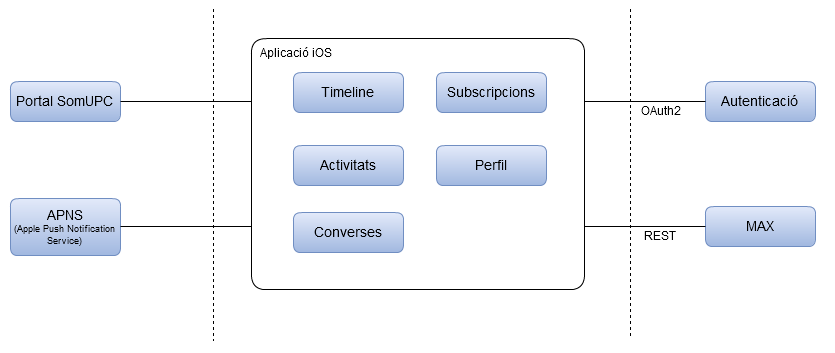
\includegraphics[scale=0.7]{Analisis/Abast/diagrama_context.png}
    \caption{Diagrama de context.}
    \label{fig:diagrama_context}
\end{figure}
\FloatBarrier

El projecte s'emmarca dintre del SomUPC, per tant és molt important delimitar les fronteres del sistema. El sistema a desenvolupar es tracta exclusivament de l'aplicació iOS, aquesta utilitzarà serveis externs, però aquests no formen part de l'abast. Al diagrama de context de la figura \ref{fig:diagrama_context} es poden veure clarament les barreres del projecte que delimiten l'abast.

L'aplicació utilitza el MAX com a font de l'activitat social, el portal SomUPC per a obtenir les fotografies dels usuaris, el APNS\footnote{Apple Push Notification Service} d'\textit{Apple} per a les notificacions \textit{push} i el servidor d'autenticació de la UPC per a l'autenticació dels usuaris.



\pagebreak
\subsection{Mètodes de validació}

Al seguir la metodologia \textit{Scrum}, no es necessita definir criteris d'acceptació de tot el projecte sencer, ja que la pròpia dinàmica ofereix un fort control del producte per part de negoci.

Un dels millors aspectes d'aquesta metodologia és la gran cohesió que crea entre tots els membres involucrats al projecte. En general sempre hi ha una mateixa visió del producte que s'està creant, i negoci pot anar perfilant el producte durant el transcurs dels \textit{sprints}.

No es defineixen criteris d'acceptació de tot el producte, però si que es defineixen criteris d'acceptació de les diferents tasques. Gràcies a que les tasques tenen una granularitat molt petita, els criteris d'acceptació poden ser molt precisos i concisos.

Com s'ha vist anteriorment, els encarregats de validar els criteris d'acceptació de les tasques són els membres de negoci, durant les reunions de demostració.

\pagebreak
\subsection{Riscs}

En aquest projecte s'han de tenir en compte els riscs involucrats al procés de desenvolupament per detectar-los el més aviat possible. Per aquest projecte s'han detectat aquests riscs:

\begin{itemize}
    \item \textbf{Producte no desitjat pel client.} Al tractar-se d'un producte destinat a un client, hi ha la possibilitat que un cop finalitzat el projecte, el client rebi un producte que no és el que esperava obtenir. Per evitar aquest risc, com s'ha indicat en els apartats anteriors, es segueix la metodologia \textit{Scrum} i per tant el client obté un \textit{feedback} continuat durant els \textit{sprints}. Si en algun moment el client detecta que el projecte no és el que espera, el client pot comunicar-ho al següent \textit{sprint} i re-orientar el projecte.
    \item \textbf{Control del temps.} Un risc molt important és excedir el termini de temps establert per a aquest projecte. Per evitar aquest risc, es farà un control exhaustiu per tal de que es compleix la planificació establerta.
    \item \textbf{Producte poc eficient.} Al tractar-se d'un producte final, destinat a tot tipus d'usuari, el producte resultant ha de tenir un bon rendiment en velocitat d'ús. Per evitar aquest risc, durant el desenvolupament del projecte es tindrà molt en compte la velocitat d'execusió.
    \item \textbf{Ús inadequat.} Com que al producte final podran accedir tot tipus d'usuari, hi ha la possibilitat que algun usuari faci un ús inadequat del producte. Per evitar aquest risc, durant el desenvolupament es tindrà en compte la seguretat de l'aplicació per evitar usos inadequats.
\end{itemize}                                    

\newpage
\cleardoublepage
\section{Especificació}


\subsection{Requisits funcionals}

En aquest projecte s'han definit els requisits funcionals seguint el model d'històries d'usuari, ja que s'ha seguit la metodologia \textit{scrum}. Cada una de les històries d'usuari descriu una funcionalitat del sistema.

\input{Memoria/Especificacio/HistoriesUsuari/histories.tex}

\input{Memoria/Especificacio/model_conceptual.tex}

\input{Memoria/Especificacio/model_comportament.tex}


\input{Memoria/Especificacio/requisits_no_funcionals.tex}







\newpage
\cleardoublepage

\section{Disseny arquitectònic}


\subsection{Patrons de disseny}

Les aplicacions iOS estan basades en \textit{Cocoa}. \textit{Cocoa} és una interfície de programació d'aplicacions natives orientada a objectes per a sistemes operatius OS X. En aquesta secció estan explicats els patrons de disseny per a aplicacions basades en \textit{Cocoa}.

\input{Memoria/Arquitectura/iOS/mvc.tex}

\input{Memoria/Arquitectura/iOS/notification.tex}

\input{Memoria/Arquitectura/iOS/categoria.tex}

\input{Memoria/Arquitectura/iOS/delegat.tex}

\input{Memoria/Arquitectura/iOS/singleton.tex}



\pagebreak
\subsection{Capa de presentació}

\input{Memoria/Arquitectura/Projecte/Presentacio/disseny_extern.tex}

\input{Memoria/Arquitectura/Projecte/Presentacio/mapa_de_navegacio.tex}


\pagebreak
\subsection{Capa de domini}

\input{Memoria/Arquitectura/Projecte/Domini/model_conceptual.tex}
\input{Memoria/Arquitectura/Projecte/Domini/model_comportament.tex}


\pagebreak
\subsection{Capa de dades}

Aquest projecte no disposa de capa de dades, ja que totes les dades les obté del servidor MAX. Aquestes dades no es guarden a l'aplicació i per tant cada cop es tanca i es torna a obrir l'aplicació, les dades es tornen a carregar del servidor.

La única informació que es guarda a l'aplicació són un conjunt de dades de l'usuari. Es persisteix el nom d'usuari i el \textit{token}, que s'obtenen a l'hora d'iniciar sessió. Aquestes dades es guarden utilitzant \textit{NSUserDefaults}\footnote{Emmagatzematge que ofereix el sistema per a guardar parelles clau-valor.}.

\pagebreak

\subsection{Model de desplegament}

El projecte d'aquest treball, forma part del SomUPC. Per aquest motiu el model de desplegament s'ha ampliat amb algunes components del model de desplegament del SomUPC per a complementar la visió de l'entorn de desplegament. A la figura \ref{fig:desplegament} el dispositiu ``Aplicació nativa'', equival a l'aplicació client del MAX iOS (objecte d'aquest treball) o al client \textit{Android} del MAX.

Els dispositius que estan directament relacions amb aquest projecte són l'aplicació nativa iOS, el servidor MAX del que s'obté la informació social, el servidor OAuth amb el que es validen els usuaris i s'obté el \textit{token} de l'usuari i el servidor SomUPC del que s'obtenen les imatges dels usuaris.

\begin{figure}[ht]
    \centering
    \includegraphics*[scale=0.7]{Memoria/Arquitectura/Projecte/desplegament.png}
    \caption{Model de desplegament.}
    \label{fig:desplegament}
\end{figure}
\clearpage


\pagebreak

\subsection{Distribució de l'aplicació}

Al tractar-se d'una aplicació iOS, el procés de distribució esta definit per \textit{Apple}. A més en aquest project s'utilitza la plataforma \textit{TestFlightApp}\footnote{Sistema de distribució de versions \textit{beta} de l'aplicació. \url{https://testflightapp.com/}} per a realitzar proves amb usuaris reals. Els passos per a desplegar una versió de l'aplicació son els següents:

\begin{enumerate}
    \item Instal·lar la versió al dispositiu a través del cable USB, i verificar el correcte funcionament.
    \item Distribuir la versió mitjançant \textit{TestFlightApp} per a que un grup d'usuari reduït (20-30 usuaris) verifiquin el correcte funcionament de la versió.
    \item Enviar la versió al sistema de distribució d'\textit{Apple}.
    \item Un cop \textit{Apple} revisa i accepta la versió, es distribueix mitjançant l'\textit{App Store} d'\textit{Apple}.
\end{enumerate}

Per tant hi han tres canals per a instal·lar l'aplicació a un dispositiu, a través de l'\textit{App Store} d'\textit{Apple}, a través de \textit{TestFlightApp} o mitjançant un cable USB. A la figura \ref{fig:distribucio} es poden veure especificats els tres canals de distribució.

\begin{figure}[ht]
    \centering
    \includegraphics*[scale=0.5]{Memoria/Arquitectura/Projecte/distribucio.png}
    \caption{Distribució de l'aplicació.}
    \label{fig:distribucio}
\end{figure}
\clearpage



\newpage
\cleardoublepage
\section{Desenvolupament}

En aquesta secció s'explica el desenvolupament del projecte, l'anàlisi i implementació de cada una de les històries d'usuari definides a l'especificació del projecte. 

Per a facilitar la comprensió, s'ha realitzat una agrupació d'històries d'usuari en etapes. Aquesta agrupació s'ha realitzat en funció de la temàtica de la història. Això no implica que s'hagi desenvolupat el projecte en l'ordre que apareixen les històries a continuació.

A la taula \ref{tab:histories_sprint} es poden veure les històries d'usuari que s'han desenvolupat a cada \textit{sprint}. A l'annex, a la secció  \ref{sec:histores_sprint}, estan les històries d'usuari per \textit{sprint} amb més detall. 


\begin{table}[ht]
    \begin{tabularx}{\linewidth}{|X|X|X|X|X|X|X|X|X|X|X|X|X|X|X|X|}
        \hline
         \textbf{1} & \textbf{2} & \textbf{3} & \textbf{4} & \textbf{5} & \textbf{6} & \textbf{7} & \textbf{8} & \textbf{9} & \textbf{10} & \textbf{11} & \textbf{12} & \textbf{13} & \textbf{14} & \textbf{15} & \textbf{16} \\
        \hline
         1	&	2\newline 3\newline 4	&	15	&	8\newline 12	&	5\newline 16	&	6	&	7\newline 17\newline 14	&	18\newline 19 & 20	&	9\newline 13	&	10\newline 11	&	23\newline 24\newline 25\newline 26	&	27	&	21	&	22 & - \\
        \hline
    \end{tabularx}
    \caption{Histories d'usuari realitzades per \textit{sprint}.}
    \label{tab:histories_sprint}
\end{table}



% Instruccions:

\begin{comment}

% Posar dues imatges:
\pintaDosImatges
    {idFoto1}
        {TextFoto1}
    {idFoto1}
        {TextFoto2}

% Posar una imatge:
% \pintaUnaImatge
%     {idFoto1}
%         {TextFoto1}

% Fer referencia a una de les fotos:
\refImatgeCaptura{idFoto}

\end{comment}



% Macros:

\newcommand{\refImatgeCaptura}[1]{\ref{fig:#1}}

\newcommand{\pintaDosImatges}[4]{
    \setlength{\fboxsep}{0pt}
    \begin{figure}[ht]
        \begin{minipage}[t]{.48\textwidth}
            \centering
            \fbox{\includegraphics[scale=0.25]{Memoria/Implementacio/Captures/#1.png}}
            \caption{#2}
            \label{fig:#1}
        \end{minipage}%
        \hfill
        \begin{minipage}[t]{.48\textwidth}
            \centering
            \fbox{\includegraphics[scale=0.25]{Memoria/Implementacio/Captures/#3.png}}
            \caption{#4}
            \label{fig:#3}
        \end{minipage}
    \end{figure}
}



\newcommand{\pintaUnaImatge}[2]{
    \setlength{\fboxsep}{0pt}
    \begin{figure}[ht]
        \centering
        \fbox{\includegraphics*[scale=0.25]{Memoria/Implementacio/Captures/#1.png}}
        \caption{#2}
        \label{fig:#1}
    \end{figure}
}


\subsection{Estructura de l'aplicació}
\label{sec:etapa1}

L'estructura de l'aplicació és la primera etapa, i prerequisit de la resta d'etapes. L'objectiu és el d'obtenir un esquelet base d'aplicació iOS per a poder implementar les funcionalitats que es demanen.
Aquesta base ha de tenir les següents funcionalitats:

\begin{compactitem}
    \item El sistema ha de demanar a l'usuari que introdueixi les seves credencials.
    \item Les dades que ha introduït l'usuari s'han de validar amb el servei d'autenticació.
    \item Si les dades són correctes s'ha d'obtenir el \textit{token} de l'usuari, si no són correctes s'ha d'informar a l'usuari del problema.
    \item El sistema ha d'establir la connexió amb el MAX amb el \textit{token} de l'usuari.
    \item El sistema ha de poder obtenir informació d'algun dels serveis del MAX, com per exemple el \textit{timeline}.
\end{compactitem}

Aquesta etapa inclou les històries d'usuari 1 i 2 (pàgina \pageref{sec:historia_1}).

\subsubsection{Implementació}
A l'iniciar aquesta etapa es partia de zero ja que era l'inici del projecte. Abans de començar a crear el projecte es va fer un petit estudi de la situació, per poder decidir quina estructura era la millor i com fer la connexió al MAX.

L'estructura de la interfície està fixa pel client que va demana que l'aplicació estigui estructura en pestanyes, i dintre de les pestanyes s'ha de navegar utilitzant la barra de navegació. 

Sobre l'estructura interna de l'aplicació es va decidir seguir els patrons habituals de disseny que proposa \textit{Apple}\cite{apple_disseny}. Aquests patrons en essència són:

\begin{itemize}
    \item \textit{Model-View-Controller} (Model-Vista-Controlador, MVC) \footnote{\url{https://developer.apple.com/library/ios/documentation/General/Conceptual/DevPedia-CocoaCore/MVC.html}}: Aquest patró de disseny s'utilitza per a estructurar tota l'aplicació.
    \item \textit{Delegation} (Delegació) \footnote{\url{https://developer.apple.com/library/ios/documentation/General/Conceptual/DevPedia-CocoaCore/Delegation.html}}: Facilita la transmissió d'informació i dades d'un objecte a un altre.
    \item \textit{Target-action} \footnote{\url{https://developer.apple.com/library/ios/documentation/General/Conceptual/Devpedia-CocoaApp/TargetAction.html}}: Patró de disseny que relaciona les interaccions de l'usuari (botons i controls) amb el codi que la aplicació ha d'executar.
    \item \textit{Block objects} \footnote{\url{https://developer.apple.com/library/ios/documentation/General/Conceptual/DevPedia-CocoaCore/Block.html}}: Utilitza blocs de codi per implementar \textit{callbacks} i codi asíncron.
\end{itemize}

Un dels punts més importants va ser prendre una decisió sobre com connectar el sistema amb el MAX. Per fer-ho es van considerar tres possibilitats:
\begin{itemize}
    \item  \textbf{Fer les crides des de l'aplicació}: consisteix en realitzar totes les consultes i modificacions des de l'aplicació i d'aquesta manera fer tot el sistema molt eficient. Aquesta solució té l'inconvenient de presentar un alt nivell d'acoblament entre l'aplicació i el MAX, i per tant, el codi resultant seria molt poc canviable.
    \item  \textbf{Implementar una llibreria}: aquesta possibilitat implica desenvolupar una llibreria externa a l'aplicació que permeti obtenir la informació del MAX mitjançant una API en Objective-C. Aquesta solució ofereix un bon nivell de canviabilitat ja que els canvis en el MAX només comportarien canvis a la llibreria. Aquesta opció implica un gran esforç de desenvolupament.
    \item  \textbf{Utilitzar una llibreria que facilit la connexió}: en aquest cas s'hauria de fer una cerca de possibles llibreries i posteriorment triar la més adient per a aquest cas. L'objectiu és delegar a la llibreria desenvolupada per un tercer la responsabilitat d'establir i mantenir la connexió amb el MAX, així com fer totes les consultes i modificacions seguint la filosofia REST. El principal inconvenient d'aquesta opció és el de limitar el desenvolupament a les funcionalitats que ofereix la llibreria.
\end{itemize}

Es va decidir descartar la primera opció ja que el producte resultant seria difícil de mantenir. Per decidir entre la segona i la tercera opció es va fer una petita cerca de llibreries de tercers.

Com a resultat de la cerca es van obtenir quatre llibreries que cumplien amb els requisits:
\begin{itemize}
    \item  ASIHTTPRequest \footnote{\url{http://allseeing-i.com/ASIHTTPRequest/}}: aquesta llibreria facilita l'establiment de connexions amb el servidor per a fer consultes oferint una API de més alt nivell que les consultes natives d'Objective-C. El problema principal d'aquesta llibreria és que no té un suport continuat ni s'adapta a les necessitats del projecte.
    \item  AFNetworking \footnote{\url{https://github.com/AFNetworking/AFNetworking}}: llibreria similar a ASIHTTPRequest, facilita l'establiment de connexions amb una API de més alt nivell que la nativa. De la mateixa manera que amb l'anterior llibreria, aquesta no és la més adient per al projecte ja que només facilita l'accés al servidor, però no facilita la implementació dels principis REST.
    \item  RestKit \footnote{\url{https://github.com/RestKit/RestKit}}: aquesta llibreria proporciona una interficie completa per a que l'aplicació es comuniqui amb un servidor REST de forma semi-transparent. És a dir que l'aplicació ha de configurar tots els mapeigs dels serveis del servidor i posteriorment l'aplicació només ha de fer les crides a RestKit, que les transformarà en crides REST.
    \item  Spaghetti \footnote{\url{https://github.com/noodlewerk/Spaghetti}}: llibreria similar a RestKit però per servidors que no utilitzen el protocol REST, per tant aquesta llibreria és més flexible que la anterior.
\end{itemize}

Després d'estudiar i analitzar totes les possibilitats es va decidir fer una prova de concepte amb la llibreria RestKit\cite{restkit}. Perquè era la que més s'ajustava a les necessitats del projecte i podia aportar més valor. 

La prova de concepte va consistir en crear el projecte de l'aplicació. Es va partir d'una plantilla d'aplicació amb pestanyes que ofereix \textit{Apple}. Es va afegir la llibreria RestKit i es va provar de configurar amb un \textit{token} del MAX posat manualment. El primer servei que es va intentar utilitzar va ser el del \textit{timeline}. Es va configurar el mapeig del servei i el mapeig del model de dades (seguint l'estàndard ActivityStream\cite{activityStream}).

Una vegada obtingudes amb èxit les dades del MAX del \textit{timeline} mitjançant la prova de concepte, es va decidir utilitzar RestKit per al projecte.

A partir d'aquí es va continuar amb el desenvolupament afegint la pantalla d'inici de sessió. Per a validar l'usuari no es va utilitzar RestKit, si no que es va fer una consulta directament amb el servei de validació de la UPC ja que aquest no funciona amb REST si no que segueix el protocol d'\textit{OAuth2}\cite{oauth2}. A la figura \ref{fig:limit_restkit} es pot veure a quins àmbits s'utilitza RestKit i a quins no s'utilitza.

\begin{figure}[ht]
    \centering
    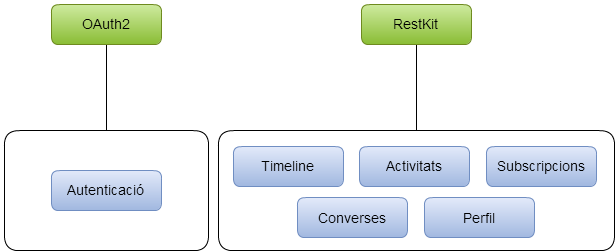
\includegraphics[scale=0.6]{Memoria/Implementacio/LimitRestKit.png}
    \caption{Limit d'ús de la llibreria RestKit.}
    \label{fig:limit_restkit}
\end{figure}


Un cop l'usuari estava validat s'obtenia el \textit{token} i ja es podia configurar RestKit amb el nom d'usuari i el \textit{token} de l'usuari que havia iniciat sessió.






\newpage
\subsection{\textit{Timeline} i veure activitat}
\label{sec:etapa2}

Aquesta etapa té com a objectiu implementar les històries d'usuari relacionades amb el \textit{timeline} i les activitats. Com la resta de les etapes, aquesta només es pot realitzar si s'ha finalitzat la primera etapa (\nameref{sec:etapa1}). En aquesta etapa s'han d'implementar les següents funcionalitats:


\begin{compactitem}
    \item El sistema ha d'obtenir i mostrar les activitats del \textit{timeline} de l'usuari.
    \item Si l'usuari selecciona una activitat al \textit{timeline}, el sistema ha de mostrar el contingut d'aquesta. Ha de poder veure el text, la data de publicació, l'autor i els comentaris de l'activitat.
    \item L'usuari ha de poder publicar un nou comentari a una activitat.
    \item L'usuari ha de poder publicar una nova activitat, indicant el text i el context al que es publica.
    \item L'usuari ha de poder esborrar una activitat i un comentari.
    \item L'usuari ha de poder publicar una imatge. El sistema ha de mostra una pre-visualització a sota del text de l'activitat.
    \item L'aplicació ha de ser capaç d'obrir fitxers des de qualsevol altra aplicació. Quan l'usuari ho realitzi, se li ha de mostrar la vista de publicació d'una activitat, indicant que està adjuntant un fitxer.
\end{compactitem}

Aquesta etapa inclou les històries d'usuari 3, 4, 5, 6, 22, 23 i 27 (pàgines \pageref{sec:historia_3} i \pageref{sec:historia_22}).

\subsubsection{Implementació}
Per completar la primera etapa es va obtenir la informació del \textit{timeline} de l'usuari. Però aquesta informació no es mostrava amb la interfície, només es mostrava per consola. En aquesta etapa aquesta informació s'havia de mostrar seguint les directrius que havia establer el client.

A la pestanya del \textit{timeline} es va afegir una taula amb les cel·les personalitzades. Es va decidir utilitzar la taula nativa d'iOS (\textit{UITableView}) per a mostrar la informació de les activitats ja que d'aquesta manera es podien aprofitar totes les funcionalitats d'aquest element (per exemple la possibilitat d'esborrar un element lliscant amb el dit cap a un costat). En aquesta cel·la es mostra el nom de l'autor de l'activitat juntament amb la seva imatge, la data de publicació i un tros del text de l'activitat.

\pintaDosImatges
    {captura-timeline}
        {Resultat de la vista del \textit{timeline}.}
    {captura-veure-activitat}
        {Resultat de la vista de veure activitat.}

Un cop es va disposar de la vista del \textit{timeline} completada, es va continuar afegint una nova vista per a mostrar la informació d'una activitat. Aquesta vista es mostra quan l'usuari clica a una cel·la al \textit{timeline}, aleshores el sistema carrega la informació de l'activitat del servidor i la mostra a l'usuari.

En aquesta nova vista, la vista de l'activitat, es mostra el nom de l'autor de l'activitat, la data de quan es va publicar i el text complert de l'activitat. Al costat d'aquesta informació es mostra la imatge de l'autor. En cas que l'activitat disposi de comentaris, aquests es mostren a sota en format de llista. 

Per a posar els comentaris també es va optar per utilitzar una taula nativa d'iOS pels mateixos motius que al \textit{timeline}.
La funcionalitat d'afegir comentaris es va implementar amb una nova finestra que es mostra quan l'usuari clica al botó ``+'' de la barra de navegació.


Aquesta vista conté un camp de text i dos botons a la barra de navegació: ``Desar'' i ``Cancel·lar''. Si l'usuari després d'introduir un text el desa, es fa la petició al servidor per afegir el comentari. Un cop el servidor ha creat el comentari l'aplicació tanca la vista d'afegir un comentari i refresca els comentaris de la vista veure activitat.


\pintaDosImatges
    {captura-publicar-comentari}
        {Resultat de la vista de publicar comentaris.}
    {captura-publicar-activitat-buit}
        {Resultat de la vista de publicar activitat.}


Les funcionalitats esborrar activitat i esborrar comentari es van afegir utilitzant la funcionalitat de les taules natives d'iOS. Detectant l'acció de l'usuari de ``lliscar'' cap a la dreta una cel·la de la taula i mostrant un botó d'esborrar. Un cop l'usuari clica el botó, el sistema demana confirmació a l'usuari, i si l'usuari accepta, el sistema realitza la petició al servidor per a realitzar l'esborrat.

Per a implementar la confirmació que demana el sistema a l'usuari, es va utilitzar un diàleg natiu d'iOS (\textit{UIAlertView}) amb dos botons, un per acceptar i l'altre per a cancel·lar.

Per a desenvolupar la funcionalitat d'afegir noves activitats, es va partir de la d'afegir comentari. Es va afegir a sobre del camp de text la informació de l'usuari i als contexts als que es publica.

El client va demanar que per triar els contexts als que publicar, es mostrés una nova vista amb la llista de contexts als que l'usuari té permís per a publicar. En aquesta vista l'usuari havia de poder fer una selecció múltiple de contexts i tornar a la vista de nova activitat.


\pintaDosImatges
    {captura-publicar-activitat-selec-context}
        {Resultat de la vista d'afegir contexts.}
    {captura-publicar-activitat-imatge}
        {Resultat de la vista de publicar una activitat amb una imatge.}

Un cop l'usuari ha introduït el contingut de l'activitat i ha seleccionat els contexts als que publicar, el sistema fa les crides necessàries per a publicar les activitats al servidor.
Per a obrir aquesta vista l'usuari ha de clicar al botó ``+'' de la barra de navegació del \textit{timeline}.

Inicialment les activitats només havien de contenir text, però gracies a utilitzar la metodologia \textit{scrum}, el client durant el transcurs del projecte va necessitar la funcionalitat d'afegir imatges/fitxers a les activitats, i per tant es va afegir com a funcionalitat requerida. Al afegir aquesta funcionalitat es van reajustar algunes funcionalitats, simplificant-les. No va ser necessari treure cap funcionalitat.

Aquest nou requisit implicava dues tasques, l'usuari havia de poder afegir una imatge des de l'aplicació (de la galeria d'imatges o de la càmera) i l'usuari havia de poder afegir fitxers des d'una altra aplicació del dispositiu. 

La primera tasca va implicar afegir dos botons a la interfície (un per la galeria i un per la càmera), que al clicar obri el diàleg natiu corresponent. Un cop l'usuari ha triat la imatge, aquesta s'afegeixi a sota del text de l'activitat en format miniatura. A més s'han de canviar els dos botons per un d'una paperera per a poder esborrar la imatge.

Per a la segona tasca, es va modificar el fitxer de configuració de l'aplicació. Es va declarar que l'aplicació pot obrir tot tipus de fitxers. A més, es va preparar l'aplicació per a que al obrir un fitxer amb l'aplicació, se li mostri a l'usuari la vista de nova activitat. A sota del camp de text de la vista, es mostra una capsa amb el nom del fitxer que s'està adjuntant.

En tots dos casos, quan l'usuari crea la nova activitat, es fan les crides corresponents al MAX per a enviar el fitxer.


\pintaDosImatges
    {captura-obrir-fitxer}
        {Adjuntar un fitxer des d'una altra aplicació.}
    {captura-adjuntar-fitxer}
        {Resultat de la vista de publicar una activitat amb un fitxer.}
\clearpage





\newpage
\subsection{Gestió de subscripcions}

L'objectiu d'aquesta etapa és el de dotar a l'aplicació la funcionalitat de gestionar les subscripcions de l'usuari. És a dir, oferir a l'usuari la possibilitat de veure les seves subscripcions, esborrar-ne una i afegir-ne de noves.

Per a considerar l'etapa com a finalitzada, l'aplicació ha de tenir les següents funcionalitats:

\begin{compactitem}
    \item El sistema ha d'obtenir i mostrar les subscripcions de l'usuari.
    \item Si l'usuari selecciona una subscripció, el sistema ha de mostrar les activitats del context seleccionat.
    \item L'usuari ha de poder buscar contexts als que es pugui subscriure.
    \item Si l'usuari ha buscat un context i el selecciona s'ha de subscriure.
    \item L'usuari ha de poder esborrar una subscripció.
\end{compactitem}

Aquesta etapa inclou les històries d'usuari 7, 8, 9, 10 i 24 (pàgines \pageref{sec:historia_7} i \pageref{sec:historia_24}).

En aquesta etapa es poden aprofitar algunes vistes definides a ``\nameref{sec:etapa2}''. Com que les etapes no impliquen un ordre, en cas que el client prioritzi aquestes funcionalitats per davant de les de l'altra etapa es realitzaran en aquesta etapa.

\subsubsection{Implementació}

El primer que es va fer va ser afegir una nova pestanya a l'aplicació i en aquesta pestanya afegir una taula amb el seu controlador. Aquesta taula obtenia les dades des les subscripcions de l'usuari i les agrupava per tipologia del context.

Per a distingir les diferents tipologies dels contexts, aquests al atribut \textit{tags} contenen una etiqueta pre-definides. A la taula \ref{tagsContexts} es poden veure les diferents etiquetes i els seus significats. Si un context no disposa de cap pre-definida, aleshores es classifica com a ``Altres''.

\begin{table}[h]
    \begin{center}
    \begin{tabular}{| l | l |}
        \hline
            \textbf{\textit{Etiqueta}}  & \textbf{Significat}           \\ 
        \hline
            {[ASSIG]}                     & Context d'una assignatura     \\ 
            {[INST]}                      & Context institucional         \\
            {[COMMUNITY]}                 & Context d'una comunitat       \\
        \hline
    \end{tabular}
    \end{center}
    \caption{ Significat de les diferents etiquetes. \label{tagsContexts}}
\end{table}

Després es va crear una nova vista similar a la del \textit{timeline} però carregant només les activitats d'un context. Aquesta vista es mostra quan l'usuari selecciona un context de la llista de subscripcions.

Gràcies a la gran similitud entre aquesta vista i la del \textit{timeline}, es va poder re-utilitzar una part de la feina feta a l'etapa ``\nameref{sec:etapa2}''. Es va utilitzar la cel·la del \textit{timeline} ja que a les dues situacions es mostrava una activitat i es necessitava mostrar la mateixa informació. Com que s'havia de tornar a mostrar la informació de l'activitat al clicar a la cel·la, també es va re-utilitzar la vista de veure una activitat.



\pintaDosImatges
    {captura-subscripcions}
        {Resultat de la vista de subscripcions.}
    {captura-subscripcio-activitats}
        {Resultat de la vista d'activitats d'un context.}


També s'havia d'oferir a l'usuari la possibilitat de publicar una activitat al context. Es va aprofitar la vista d'afegir una activitat fent una petita modificació per a poder obrir la vista amb un context ja seleccionat.

Per acabar aquesta etapa, s'havia de poder esborrar una activitat i una subscripció a les activitats d'un context i a la vista de les subscripcions respectivament. Per fer-ho es va seguir la forma en que s'ha definit anteriorment.



\newpage
\subsection{Converses}
\label{sec:fase4}

L'objectiu d'aquesta etapa és el d'afegir les converses privades entre els usuaris. S'han d'implementar les següents funcionalitats:

\begin{compactitem}
    \item El sistema ha d'obtenir i mostrar les converses de l'usuari.
    \item Si l'usuari selecciona una conversa, el sistema ha d'obtenir tots els missatges i mostrar-los a l'usuari en format de xat.
    \item L'usuari ha de poder publicar un nou missatge a una conversa.
    \item L'usuari ha de poder veure la informació d'una conversa (nom i participants) i modificar-ho si és el creador de la conversa.
    \item L'usuari ha de poder crear una nova conversa indicant els participants i el contingut del primer missatge. En cas que hi hagi més de dos participants, el sistema ha de demanar a l'usuari el nom del grup.
    \item L'usuari ha de poder sortir d'una conversa o esborrar-la si és el creador.
\end{compactitem}

Aquesta etapa inclou les històries d'usuari 14, 15, 16, 17, 18, 19 i 25 (pàgines \pageref{sec:historia_14} i \pageref{sec:historia_25}).

S'ha separat en una altra etapa les millores a les converses de temps real i notificacions \textit{push}. Aquesta separació és deguda a que ajuntar-les amb aquesta etapa complicaria molt aquest apartat. Per aquest motiu s'ha considerat separar-ho en dues etapes. Això no implica que al projecte s'hagin d'implementat per separat.

\subsubsection{Implementació}

La vista de les converses igual que la del \textit{timeline} i les subscripcions mostra una llista de elements, en aquest cas converses, per tant el format ideal és el d'una taula.

Per a les converses es va haver d'afegir un nou tipus de cel·la amb la informació de la conversa (nom, text i data de l'últim missatge, i la fotografia de l'usuari/grup).

\pintaDosImatges
    {captura-converses}
        {Resultat de la vista de converses.}
    {captura-conversa-missatges}
        {Resultat de la vista dels missatges d'una conversa.}

La tasca principal d'aquesta etapa va ser la de desenvolupar la vista de la conversa, amb l'estil de xat. Per a fer-ho es van valorar diverses opcions. Es va fer una petita cerca de projectes que haguessin necessitat implementar un xat/SMS, i tutorials que parlessin del tema. El resultat va ser que hi havien molts projectes, molts d'ells amb el codi obert.

El projecte que més s'ajustava a les necessitats d'aquest projecte va ser \textit{AcaniChat}\footnote{https://github.com/acani/AcaniChat}. Però integrar els components d'\textit{AcaniChat} amb els del projecte no era senzill, així que es va decidir seguir els passos que havien seguit els desenvolupadors d'aquesta llibreria, ja que al \textit{ReadMe} d'aquesta citaven les fonts.

Per aquest motiu es va seguir el tutorial \textit{Tutorial on SMS style bubbles}\cite{bubbles_tutorial}. Després de seguir-lo i obtenir les bafarades amb un text, es va modificar per ajustar les bafarades amb els requisits del client. Aquest volia que es mostres l'autor (si no era el mateix usuari) i la data de publicació a més del contingut del missatge.

Un cop ja es tenia la vista preparada només faltava preparar les crides per a carregar la informació del servidor.

Des de la vista d'una conversa clicant un botó de la barra de navegació, s'ha de mostrar una nova finestra amb les dades de la conversa. A més, en cas que es tracti d'una conversa de grup i l'usuari sigui el creador de la conversa, també ha de poder modificar el nom del grup i afegir/treure participants. 

\pintaDosImatges
    {captura-editar-conversa-propietari}
        {Resultat de la vista d'informació d'una conversa (com a propietari).}
    {captura-editar-conversa-editant}
        {Resultat de la vista d'editar la informació d'una conversa.}

Per oferir aquesta funcionalitat, es va afegir una nova vista modal amb el nom de la conversa i una llista de participants. Com que a la llista hi havia possibilitats que es poguessin eliminar participants de la conversa es va utilitzar una taula nativa d'iOS. Es va crear una nova vista de cel·la per a poder mostrar la fotografia de l'usuari, el seu nom i una etiqueta indicant si és el propietari o no.

Si l'usuari és el creador de la conversa pot esborrar un usuari, lliscant la cel·la del participant cap a un costat. Aleshores la cel·la es desplaça cap a un costat i apareix un botó d'esborrar. Si l'usuari clica al botó se li mostra un confirmació i si aquest ho accepta s'esborra el participant de la conversa.

En cas que l'usuari tingui permís per editar la conversa, al costat del nom del grup li apareix una icona d'un llapis. Si l'usuari clica a sobre del nom o del llapis, activa el mode d'edició. 

En aquest mode l'etiqueta del nom de la conversa desapareix i es canvia per un camp de text. Però a més de poder editar el nom també pot afegir nous participants. Per fer-ho a la barra de navegació hi ha un botó amb un ``+'', quan l'usuari el clica se li mostra una vista modal amb un camp de cerca. 

A la cerca, al mateix moment que l'usuari va escrivint el nom, el sistema realitza consultes i va mostrant el resultat a l'usuari. Un cop l'usuari selecciona un usuari de la llista de resultats, la vista de cerca es tanca. Aleshores es mostra un diàleg de confirmació per verificar que l'usuari realment vol afegir al membre. 

\pintaDosImatges
    {captura-nova-conversa}
        {Resultat de la vista de nova conversa.}
    {captura-cercar-usuaris}
        {Resultat de la vista de cercar usuaris.}

La vista de cerca de persones es va desenvolupar com a component independent, per a poder ser re-utilitzat fàcilment (per exemple al crear una nova conversa). Per fer-ho, es va fer que el controlador de la vista retornés el \textit{username} mitjançant una notificació (amb el \textit{NSNotificationCenter}), i que la vista que havia instància el cercador estigués registrat com a observador de la notificació. 
        
A la barra de navegació de la llista de converses, hi ha un botó ``+'' per a crear una nova conversa. En aquest cas, se li mostra una vista modal amb un camp de text per a introduir el contingut del primer missatge. A més a sobre d'aquest camp hi ha un camp per a afegir participants.

Els participants es poden afegir escrivint els noms d'usuari o clicant al botó ``+''. En aquest últim cas, el sistema mostra la vista de cercar usuaris (la mateixa que s'utilitza per afegir persones al editar una conversa).

A la llista de converses l'usuari pot esborrar o sortir d'una conversa, lliscant cap a un costat la cel·la. Un cop ho ha realitzat, el sistema mostra un botó d'esborrat. Abans d'esborrar la conversa, el sistema demana una confirmació a l'usuari.























\newpage
\subsection{Perfil}

L'objectiu d'aquesta etapa és el d'oferir a l'usuari la possibilitat de veure el seu perfil i gestionar-lo.  S'inclouen les següents funcionalitats:

\begin{compactitem}
    \item El sistema ha d'obtenir les dades de l'usuari i les seves activitats.
    \item Si l'usuari selecciona una activitat, el sistema ha de mostrar el contingut i els comentaris de l'activitat.
    \item L'usuari ha de poder modificar les seves dades personals (nom i nom d'usuari del \textit{Twitter}.
    \item L'usuari ha de poder tancar la sessió.
\end{compactitem}

Aquesta etapa inclou les històries d'usuari 11, 12, 13, 26 (pàgines \pageref{sec:historia_11} i \pageref{sec:historia_26}).

En aquesta etapa es poden aprofitar algunes vistes definides a \nameref{sec:etapa2}. Com que les etapes no impliquen un ordre, en cas que el client prioritzi aquestes funcionalitats per davant de les de l'altra etapa es realitzaran en aquesta etapa.

\subsubsection{Implementació}

La primera tasca d'aquesta etapa és la d'afegir una nova pestanya ``Pefil'' amb el seu controlador de vista.

En aquesta vista s'ha de mostrar la informació de l'usuari conjuntament amb la seva imatge. Per tant s'ha de carregar del MAX el perfil de l'usuari. Un cop està carregat s'ha de mostrar el nom, el nom d'usuari i el \textit{twitter} de l'usuari.

\pintaDosImatges
    {captura-perfil}
        {Resultat de la vista del perfil.}
    {captura-perfil-editant}
        {Resultat de la vista del perfil en mode d'edició.}
        
A continuació s'han de mostrar les activitats publicades per l'usuari. Per fer-ho, seguint el patró definit prèviament, es va afegir una taula amb les cel·les personalitzades (re-utilitzant les del \textit{timeline}). Es fa afegir la interacció de seleccionar una cel·la que obrira la vista de veure activitat.

També es va afegir la interacció per esborrar les activitats, lliscant la cel·la cap a un costat. Quan l'usuari realitza aquesta acció, abans d'esborrar l'activitat, se li demana una confirmació per evitar esborrats accidentals.

El client va demanar que es pogués modificar el perfil de l'usuari. Per a fer-ho, es va establir que al costat del nom s'ha d'afegir una icona d'un llapis. Al clicar a sobre, la vista s'ha de transformar i a on abans es mostrava el nom ara s'ha de mostrar un camp de text amb el nom. De la mateixa manera s'ha de poder canviar el \textit{twitter}.


Quan el mode d'edició està activat, a la barra de navegació s'ha de mostrar un botó de cancel·lar i un de guardar. Si l'usuari clica al primer, s'han de descartar els canvis. Però si l'usuari clica al de guardar, s'ha de fer la modificació al servidor per a modificar el perfil de l'usuari amb els canvis introduïts per l'usuari. 

Quan no està activat el mode d'edició, s'ha de mostrar un botó a la barra de navegació per a poder tancar la sessió de l'usuari. Un cop tancada la sessió, s'ha de mostrar la vista d'iniciar sessió.

\pintaDosImatges
    {captura-perfil-sortir-confirmacio}
        {Missatge de confirmació abans de tancar sessió.}
    {captura-login}
        {Resultat de la vista d'iniciar sessió.}

\clearpage


\newpage
\subsection{Ampliació converses}

Aquesta etapa realment és una continuació de l'etapa de ``\nameref{sec:fase4}'', ja que s'afegeixen dues funcionalitats a les converses privades entre els usuaris. Les funcionalitats a desenvolupar són les següents:

\begin{compactitem}
    \item El sistema ha de notificar a l'usuari quan es publiqui un missatge a una conversa de l'usuari i aquest tingui l'aplicació tancada.
    \item Han d'arribar els missatges en temps real quan l'usuari tingui l'aplicació oberta.
\end{compactitem}

Aquesta etapa inclou les històries d'usuari 20 i 21 (pàgina \pageref{sec:historia_20}).

\subsubsection{Implementació}

Aquesta etapa està formada per dues grans tasques. Les dues funcionalitats tenen l'objectiu d'avisar a l'usuari quan un altre membre ha enviat un missatge a una conversa de l'usuari. La gran diferencia és la forma en que s'ha de notificar segons si té l'aplicació oberta o no.

Quan l'usuari té l'aplicació oberta, el missatge ha d'arribar en temps real, el dispositiu ha de vibrar i s'ha de mostrar a les vistes que ha arribat el missatge. Si l'usuari té oberta la conversa, ha de sortir el missatge a la llista de missatges. Si l'usuari no té oberta la conversa, s'ha de posar una icona a la pestanya de converses. Aquesta icona ha d'indicar el número de converses que tenen missatges sense llegir.

En canvi, quan l'usuari no té l'aplicació oberta, se li ha d'enviar una notificació \textit{push} al seu dispositiu. Aquesta notificació ha de tenir la icona, el nom de l'aplicació, i l'inici del contingut del missatge que ha arribat.

Per a desenvolupar la primera tasca, la tasca que implica afegir el temps real, es va començar analitzant el sistema que el client ja tenia implementat i quines opcions existien per poder-ho adaptar a l'aplicació iOS del projecte.

El client UPCnet ja tenia implementat el sistema utilitzant \textit{websockets}\footnote{Tecnologia que proporciona un canal de comunicació bi-direccional i \textit{full-duplex} sobre un únic \textit{socket} TCP}. Normalment a una aplicació nativa que es comunica amb un servidor s'utilitzen \textit{sockets}\footnote{Mecanisme per a l'entrega de paquets de dades provinents de la targeta de xarxa als processos. Queda definit per una parella de direccions IP local i remota, un protocol de transport i una parella de números de port local i remot.}, ja que el fet d'utilitzar \textit{websockets} afegeix capes al procés i per tant redueix l'eficiència.

Però com que el client ho va triar per a poder-ho utilitzar amb el \textit{widget} web del MAX, i aquest no podia treballar amb \textit{sockets}, o es mantenien les dues tecnologies o es treballava amb \textit{websockets}. El client va desestimar la primera opció per evitar haver de mantenir les dues tecnologies alhora.

El sistema que el client tenia implantant utilitzava el protocol \textit{STOMP}\footnote{Protocol de missatgeria orientat a missatges de text. Té l'objectiu de facilitar la compatibilitat de la missatgeria entre els llenguatges i les plataformes. Documentació\cite{stomp_doc}} per sobre dels \textit{websockets}. Es va fer una cerca de llibreries que facilitessin l'us d'aquesta combinació de protocol i tecnologia, però no es va trobar cap.

Es va trobar una llibreria que facilitava l'us de \textit{websockets} amb el llenguatge Objective-c, SocketRocket\footnote{\url{https://github.com/square/SocketRocket}}. En concret aquesta llibreria oferia una API similar a l'API nativa de \textit{sockets} d'Objective-c.

També es va trobar una llibreria client d'\textit{STOMP} però que treballava amb \textit{sockets}, objc-stomp\footnote{\url{https://github.com/juretta/objc-stomp}}. Aquesta llibreria oferia una implementació completa del protocol \textit{STOMP} per a Objective-c. Com s'ha dit prèviament, aquesta llibreria no ens servia ja que el nostre client tenia implementat el servidor amb \textit{websockets}.

Com que les dues llibreries eren codi obert i es disposava el codi al \textit{GitHub}, es va decidir re-implementar el codi de la segona (obj-stomp) per a que utilitzes \textit{websockets}. Per a fer-ho es va realitzar un \textit{fork} del projecte de \textit{GitHub} d'obj-stomp\footnote{\url{https://github.com/nmaletm/objc-stomp}}.

En aquest \textit{fork}, es va canviar les crides de \textit{sockets} per crides a la llibreria SocketRocket. Es van haver de fer alguns canvis a la constructora de la llibreria, ja que el \textit{socket} necessita una IP i un port, en canvi el \textit{websocket} necessita una direcció web. Un cop es va tenir la modificació de la llibreria, es va publicar al \textit{GitHub} per a compartir-ho amb la comunitat de desenvolupadors.

A l'aplicació per a fer la gestió del temps real, es va decidir implementar una classe controladora del temps real (\textit{UPCRealTimeManager}). Aquesta classe té la responsabilitat d'iniciar la connexió de temps real amb el servidor, i al rebre un missatge notificar-ho a la resta de l'aplicació. A més també és el responsable de tenir el control dels missatges que l'usuari no ha llegit.

Per realitzar aquesta notificació, es va decidir utilitzar el centre de notificacions. Es va crear un tipus de notificació de nou missatge, que a dintre portava com a contingut el nou missatge. 

Totes les vistes que han de fer alguna acció al rebre un missatge, es registren com a observadores del tipus de notificació de nou missatge. Quan el centre de notificacions rep una notificació de nou missatge, aquest notifica a totes classes observadores.


\pintaUnaImatge
    {captura-converses-missates-nous}
    {Llista de converses amb una conversa amb missatges sense llegir.}


D'aquesta manera, cada vista definia el seu comportament al arribar un missatge. Per exemple, el controlador de la vista de veure conversa, al rebre un nou missatge, l'afegeix a la llista de missatges. A més aquest controlador cada cop que l'usuari veu una conversa, avisa al controlador de temps real que s'han vist els missatges d'aquella conversa.

Una altra vista que també depèn dels missatges nous, és la de llista de converses. Cada cop que arriba un nou missatge, aquesta marca la conversa com a conversa amb missatges sense llegir.

L'altre tasca d'aquesta etapa és la de rebre notificacions \textit{push}. Aquesta tasca implica algunes accions per part de l'aplicació, però la majoria de tasques les ha de realitzar el servidor MAX.

En concret, l'aplicació l'únic que ha de realitzar és registrar i des-registrar l'identificador del dispositiu al MAX. Això és degut a que el MAX per poder enviar les notificacions necessita saber l'identificador del dispositiu al que ha d'enviar la notificació.

Aquest registre depèn del dispositiu i de l'usuari. Per tant, cada cop que s'inicia sessió s'ha de afegir l'identificador al MAX per al usuari que ha iniciat sessió. De la mateixa manera, cada cop que es tanca la sessió, s'ha de treure l'identificador de l'usuari al MAX.

Però abans de poder afegir o treure l'identificador al MAX, aquest s'ha d'obtenir. Per fer-ho es va preparar el \textit{UPCAppDelegate} (delegat de totes les responsabilitats generals de l'aplicació), per a que sol·licités l'identificador i al rebre el guardés per a posteriors usos. Aquest identificador en aquest moment encara no estava vinculat a cap usuari, només estava vinculat al dispositiu.

Un cop ja es disposava de l'identificador, s'havia de preparar l'aplicació per a que al iniciar sessió i al tancar-la, registres/des-registres l'identificador al MAX al usuari.

També es va preparar el \textit{UPCAppDelegate} per a que al rebre una notificació obris la pestanya de converses.

A partir d'aquest moment l'aplicació ja podia rebre les notificacions \textit{push}.









\newpage
\cleardoublepage

\section{Línies de futur} 

Aquest projecte ha estat l'inici d'una aplicació que encara té molt camí per recórrer. És una de les peces del SomUPC i per tant alhora que aquest creixi, l'aplicació també ho farà. Aquest sistema s'implantarà properament a la Universitat Politècnica de Catalunya de mà de l'aplicació Android.

A més el client UPCnet implantarà imminentment el sistema a dues organitzacions, i continuarà buscant noves organitzacions a on implantar el sistema.

Particularment al projecte d'aquest treball, s'ha de continuar treballant afegint tots els canvis i millores que es facin al MAX. Així com arreglar tots els possibles problemes que es trobin a l'aplicació. Una altra gran evolució que aportarà molt valor a l'aplicació és afegir persistència.

Actualment si no hi ha connexió a Internet, l'usuari no pot veure cap dada a l'aplicació. Afegint persistència, es podria mostrar a l'usuari la informació que anteriorment s'hagués descarregat l'aplicació, en cas que aquest no tingués accés a la xarxa. També es podria mostrar informació antiga a l'usuari mentre que la nova es descarrega, especialment si l'usuari utilitza una connexió lenta a Internet. 


\newpage
\cleardoublepage

\section{Conclusions}

Vaig començar aquest projecte sense saber que acabaria sent el meu Treball Final de Grau, durant la meva estada com a becari al inLab FIB. Aproximadament a mig projecte l'Albert hem va oferir l'oportunitat de presentar-ho com a treball i després de fer tots els tràmits amb una setmana em vaig trobar immers a l'assignatura de GEP (Gestió de Projectes).

Abans de l'inici d'aquest projecte havia desenvolupat unes quantes aplicacions natives d'iOS, però mai m'havia trobat amb un projecte d'aquesta envergadura i abast. Estic molt content ja que m'ha ofert la possibilitat de veure créixer una aplicació des de zero i veure com organitzar l'estructura interna d'aquesta. Estic segur que es podria haver fet molt millor, però estic content del resultat obtingut.

Un altre aspecte que m'ha agradat molt d'aquest projecte, és que alhora que creixia l'aplicació iOS també ho feia l'aplicació Android. Gracies a que les dues evolucionaven a un ritme igual, els membres de l'equip, hem pogut comparar com afronten els mateixos problemes els dos sistemes. Ens hem adonat com, tot hi que puguin semblar iguals, els dos sistemes tenen plantejaments molt diferents i a vegades difícil fins i tot de comparar. En algunes ocasions hem pogut solucionar problemes d'un sistema aplicar patrons de l'altre sistema.

Al projecte SomUPC hem aplicat la metodologia \textit{Scrum} i crec que ha estat una de les claus que han facilitat l'èxit del projecte. Al iniciar el projecte, teníem dues grans peces, el portal SomUPC i les aplicacions natives clients del MAX.

Al inici es va prioritzar més el portal, però es va donar un punt en que les prioritats del client van canviar i es va prioritzar completament les aplicacions. Inclús durant un període de temps, es paralitzar el portal fins acabar les aplicacions. 

Aquest canvi, sota el meu punt de vista, era necessari fer-ho, ja que el client per motius de negoci necessitava les aplicacions. Si no hagués estat per la flexibilitat de la metodologia potser no hauria estat possible. Si no s'hagués fet, el client segurament no s'hauria pogut queixar ja que el pacte inicial no contemplava el canvi. Però el fet de ser flexibles i adaptar-nos al client ha fet que aquest estigui content amb el projecte i li pugui donar continuïtat.

En aquest projecte hem treballat conjuntament l'equip SomUPC i UPCnet. Hem realitzat moltes reunions, l'experiència obtinguda en aquestes reunions és la major aportació que m'emporto d'aquest projecte. Estic segur que això m'aportarà molt al meu futur professional. Quan acabi la carrera i m'enfronti a la primera reunió de treball agrairé haver realitzat aquest projecte. Encara recordo la primera reunió que vam fer, i els nervis que vaig passar abans de començar.

Per acabar, m'agradaria agrair a tots els membres que han col·laborat en aquest projecte, tot l'equip SomUPC i l'equip d'UPCnet (negoci i equip tècnic).


\newpage
\cleardoublepage
\section{Referencies}
\nocite{*}
\bibliographystyle{unsrtnat}

\begingroup
\renewcommand{\section}[2]{}%
\bibliography{GEP/Referencies/bilbio}
\endgroup

\newpage
\cleardoublepage
\section{Annex}


\subsection{Glossari}


\textbf{Activitat}: al projecte SomUPC, és un conjunt d'informació que vol publicar un usuari a un context (o un grups de contexts) concrets. Pot ser un text, una imatge o un fitxer qualsevol.

\textbf{\textit{Activity Stream}} \cite{activityStream}: és una especificació per protocols de flux d'activitat, que s'utilitzen per a fer re-difusió de les activitats generades en serveis socials.

\textbf{APNS - \textit{Apple Push Notification Service}}: és un servei creat per \textit{Apple Inc}, que va ser llançat amb el iOS 3.0 el 17 de juny de 2009. El servei utilitza la tecnologia \textit{push} per enviar notificacions dels servidors d'aplicacions de tercers als dispositius \textit{iOS}, les notificacions poden incloure logotips, cançons o alarmes de text personalitzades.

\textbf{Context}: al projecte SomUPC, és un conjunt de persones que comparteixen alguna característica en comú, per exemple tots els alumnes d'una assignatura o tots els membres d'una facultat.

\textbf{\textit{Daily scrum}}: reunió diària de 10 minuts de l'equip de desenvolupament, per revisar les tasques realitzades el dia anterior i planificar les tasques a fer durant el dia.

\textbf{MVC - Model vista controlador}: patró de disseny per al desenvolupament de programari que separa el model de dades, la interfície usuari i la lògica de control.

\textbf{Negoci}: client del producte. Negoci està representat pel \textit{product owner} dintre de \textit{Scrum}.

\textbf{Notificació push}: descriu un estil de comunicacions a Internet on la petició d'una transacció s'origina en el servidor. Al contrari a la tecnologia pull, on la petició és originada en el client-servidor.

\textbf{\textit{Product owner}}: representa la veu del client. S'assegura que el resultat del treball de l'equip de Scrum s'adequa des de la perspectiva del negoci. El Product Owner escriu històries d'usuari i les prioritza.

\textbf{\textit{Scrum}}: marc de treball per a la gestió de projectes que defineix un conjunt de pràctiques, on cada persona participant assumeix un rol (\textit{Scrum master}, \textit{Product owner} i equip de desenvolupament), fet que permet adaptar-se a les necessitats i preferències de cada equip o organització.

\textbf{Scrum master}: facilitador del \textit{Scrum}, la feina principal del qual és eliminar els obstacles que impedeixen que l'equip arribi a l'objectiu de cada \textit{Sprint}.

\textbf{Sprint}: període en el que es realitza l'increment del producte, idealment aquest periode te una durada fixa. La durada fixa té com a objectiu mantenir un ritme constant i facilitar que l'abast dels requeriments associats es respecti per part del client durant la seva execució. 

\textbf{\textit{Sprint planning}}: reunió al inici de cada \textit{Sprint} on es decideix, valora i prioritza les tasques que entren al \textit{Sprint}.

\textbf{Subscripció}: acció que realitza l'usuari per rebre al seu \textit{timeline} totes les activitats d'un context.

\textbf{\textit{Timeline}}: espai on l'usuari pot veure totes les activitats que s'han publicat al sistema als contexts on està subscrit.

\textbf{Vista modal}: pantalla que es mostra per sobre de totes les pantalles actives. Si la pantalla que mostra la vista modal té una barra de navegació, la nova vista es superposa i cobreix la pantalla anterior, inclosa la barra de navegació.

\newpage

\subsection{Històries d'usuari per \textit{sprint}}
\label{sec:histores_sprint}

A continuació es poden veure les històries d'usuari que s'han realitzat a cada \textit{sprint}. Aquesta tria l'ha fet negoci en funció de les històries que s'han considerat que aporten més valor al projecte.

\newcommand{\pintarHistoresSprint}[1]{
    \textbf{\textit{Sprint} \arabic{numeroSprint}}\\
    #1
    \stepcounter{numeroSprint}
}

\newcounter{numeroSprint}\stepcounter{numeroSprint}

\pintarHistoresSprint
    {1. Iniciar sessió.}
    
\pintarHistoresSprint
    {26. Tancar sessió.\\
2. Veure timeline.\\
3. Veure activitat.}
    
\pintarHistoresSprint
    {14. Veure converses usuari.}
    
\pintarHistoresSprint
    {7. Veure subscripcions.\\
11. Veure perfil usuari.}
    
\pintarHistoresSprint
    {4. Veure comentaris d'una activitat.\\
15. Veure missatges d'una conversa.}
    
\pintarHistoresSprint
    {5. Crear una activitat.}
    
\pintarHistoresSprint
    {6. Afegir un comentari.\\
13. Modificar dades perfil usuari.\\
16. Afegir un nou missatge a una conversa.}
    
\pintarHistoresSprint
    {17. Visualitzar dades d'una conversa.\\
18. Modificar dades d'una conversa.}
    
\pintarHistoresSprint
    {19. Crear una conversa.}
    
\pintarHistoresSprint
    {8. Veure activitats d'una subscripció.\\
12. Veure activitats d'un usuari.}
    
\pintarHistoresSprint
    {9. Afegir una subscripció.\\
10. Cercar contexts públics.}
    
\pintarHistoresSprint
    {22. Esborrar una activitat.\\
23. Esborrar un comentari.\\
24. Esborrar una subscripció.\\
25. Sortir/Esborrar una conversa.}
    
\pintarHistoresSprint
    {27. Publicar un arxiu a una activitat.}
    
\pintarHistoresSprint
    {20. Notificacions de converses.}
    
\pintarHistoresSprint
    {21. Converses en temps real.}

    
\pintarHistoresSprint
    {Arreglar problemes i acabar coses pendents.}
    
\newpage
\subsection{Llista d'ObjectTypes}

\input{NotDef/ConfigurarCodiJSON.tex}

\begin{lstlisting}[caption=ObjectType activity, label=objectType_activity, language=json]
{
    "generator": null,
    "contexts": [{
        "url": "http://atenea.upc.edu/local/max/max/goto.php?path=/1/167/424",
        "hash": "7615301bea3d2c6f35289cae3eeba4fa073d634d",
        "displayName": "Introducci\u00f3n a la atenci\u00f3n efectiva al cliente",
        "objectType": "context"
    }],
    "object": {
        "content": "Dia 10 blended cajero",
        "objectType": "note"
    },
    "actor": {
        "username": "william.learn",
        "displayName": "William Learn",
        "objectType": "person"
    },
    "commented": "2013-11-07T22:31:05Z",
    "published": "2013-11-07T22:31:05Z",
    "verb": "post",
    "deletable": true,
    "replies": [],
    "id": "527c14a94496402db22fd7c6",
    "objectType": "activity"
}
\end{lstlisting}

\begin{lstlisting}[caption=ObjectType person, label=objectType_person, language=json]
{
    "username": "william.learn",
    "iosDevices": ["646a298e8b048bf105....d3f05c6ef976391d0"],
    "displayName": "William Learn",
    "talkingIn": [],
    "creator": "restricted",
    "id": "525f994f4496401b809afa31",
    "androidDevices": [],
    "owner": "restricted",
    "subscribedTo": [],
    "last_login": "2013-10-17T08:01:19Z",
    "published": "2013-10-17T08:01:19Z",
    "following": [],
    "objectType": "person"
}
\end{lstlisting}

\begin{lstlisting}[caption=ObjectType context, label=objectType_context, language=json]
{
    "displayName": "Habilidades directivas I: gesti\u00f3n de la resistencia y la planificaci\u00f3n",
    "tags": [],
    "url": "http://atenea.upc.edu/max/max/goto.php?path=/1/146/437",
    "creator": "restricted",
    "id": "527b77c54496402db22fd78e",
    "published": "2013-11-07T11:21:41Z",
    "owner": "restricted",
    "hash": "578345a23a56daf7a09a0a0b1ff45dccc48b4206",
    "permissions": {
        "read": "public",
        "write": "subscribed",
        "invite": "restricted",
        "subscribe": "public"
    },
    "objectType": "context"
}
\end{lstlisting}

\begin{lstlisting}[caption=ObjectType conversation, label=objectType_conversation, language=json]
 {
    "displayName": "steve.talk, william.learn",
    "creator": "william.learn",
    "messages": 1,
    "id": "526e63e0449640094a598fcf",
    "objectType": "conversation",
    "participants": ["steve.talk",
    "william.learn"],
    "lastMessage": {
        "content": "Test",
        "published": "2013-10-28T13:17:20Z"
    },
    "published": "2013-10-28T13:17:20Z",
    "owner": "william.learn",
    "permissions": {
        "read": "subscribed",
        "write": "subscribed",
        "unsubscribe": "public",
        "invite": "restricted",
        "subscribe": "restricted"
    }
}
\end{lstlisting}

\begin{lstlisting}[caption=ObjectType message, label=objectType_message, language=json]
{
	"generator": null,
	 "contexts": [{
		"participants": ["steve.talk",
		 "william.learn"],
		 "displayName": "steve.talk,
		 william.learn",
		 "id": "526e63e0449640094a598fcf",
		 "objectType": "conversation"
	}],
	 "object": {
		"content": "Test",
		 "objectType": "note"
	},
	 "actor": {
		"username": "william.learn",
		 "displayName": "William Learn",
		 "objectType": "person"
	},
	 "commented": "2013-10-28T13:17:20Z",
	 "published": "2013-10-28T13:17:20Z",
	 "verb": "post",
	 "replies": [],
	 "id": "526e63e0449640094a598fd2",
	 "objectType": "message"
}
\end{lstlisting}

\begin{lstlisting}[caption=ObjectType comment, label=objectType_comment, language=json]
{
    "content": "En Peru",
    "deletable": true,
    "published": "2013-11-08T16:15:32Z",
    "id": "527d0e244496402db22fd7d6",
    "actor": {
        "username": "william.learn",
        "displayName": "William Learn",
        "objectType": "person"
    },
    "objectType": "comment"
}
\end{lstlisting}


\newpage
\subsection{MAX}
\label{sec:max}

MAX és un sistema de recollida i visualització de registres d’activitat generada per usuaris i aplicacions així com les interactuacions entre usuaris i entre usuaris i aplicacions.

El MAX registra l’activitat de dues maneres: Activa i passiva. Quan ho fa de manera passiva, els usuaris i aplicacions que generen activitat, usen l’API del MAX per registrar-hi activitat. Quan ho fa de manera activa, el MAX va a buscar l’activitat al sistema que la genera a través d’unes regles predefinides, per exemple, l’activitat generada per un compte de Twitter i un hashtag associat.

Tant els usuaris com les aplicacions que puguin interactuar amb el MAX poden ser d’origen en escenaris corporatius (interns) o en canvi ser totalment externs al sistema.

Aquest sistema disposa d'una API REST que està protegida amb OAuth2. Aquesta API està documentada a \url{http://max.beta.upcnet.es/docs/v3/ca/}.

El codi del projecte MAX està disponible al GitHub \url{https://github.com/UPCnet/maxserver}


%\newpage
%
\subsection{Diagrama de Gantt}
\label{sec:diagrama_de_gantt}

\begin{figure}[ht]
 \centering
  \fbox{
   \scalebox{0.5}{\includegraphics*[viewport=0 0 800 910]{GEP/Annex/diagrama_gantt_v2.png}}
  }
\end{figure}

\begin{figure}[ht]
 \centering
  \fbox{
   \scalebox{0.5}{\includegraphics*[viewport=800 0 1600 910]{GEP/Annex/diagrama_gantt_v2.png}}
  }
\end{figure}

\begin{figure}[ht]
 \centering
  \fbox{
   \scalebox{0.5}{\includegraphics*[viewport=1600 0 2400 910]{GEP/Annex/diagrama_gantt_v2.png}}
  }
\end{figure}

\begin{figure}[ht]
 \centering
  \fbox{
   \scalebox{0.5}{\includegraphics*[viewport=2400 0 3200 910]{GEP/Annex/diagrama_gantt_v2.png}}
  }
\end{figure}

\begin{figure}[ht]
 \centering
  \fbox{
   \scalebox{0.5}{\includegraphics*[viewport=3200 0 4000 910]{GEP/Annex/diagrama_gantt_v2.png}}
  }
\end{figure}

\begin{figure}[ht]
 \centering
  \fbox{
   \scalebox{0.5}{\includegraphics*[viewport=4000 0 4800 910]{GEP/Annex/diagrama_gantt_v2.png}}
  }
\end{figure}

\begin{figure}[ht]
 \centering
  \fbox{
   \scalebox{0.5}{\includegraphics*[viewport=4800 0 5600 910]{GEP/Annex/diagrama_gantt_v2.png}}
  }
\end{figure}
\FloatBarrier

   





\end{document}
